%input macros (i.e. write your own macros file called MacroFile1.tex)
%% Personal macros
\newcommand{\JENC}{Jens Enzo Nyby Christensen}
\newcommand{\email}{jens@jensenzo.com}
%PhD thesis support site
\newcommand{\siteURL}{\url{www.something.com}}

%% Editing macros
\newcommand{\todo}[1]{\textcolor{red}{@TODO: #1}}
\newcommand{\sound}[1]{\textcolor{blue}{@Sound file: #1}}

%% Maths macros
\newcommand{\argmin}[1]{\underset{#1}{\mathrm{argmin}}}
\newcommand{\argmax}[1]{\underset{#1}{\mathrm{argmax}}}
\newcommand{\ttt}[1]{\times 10^{#1}}

%% Functional short-hands and inserts
\newcommand{\PdfPsText}[2]{
  \ifpdf
     #1
  \else
     #2
  \fi
}

\newcommand{\IncludeGraphicsH}[3]{
  \PdfPsText{\includegraphics[height=#2]{#1}}{\includegraphics[bb = #3, height=#2]{#1}}
}

\newcommand{\IncludeGraphicsW}[3]{
  \PdfPsText{\includegraphics[width=#2]{#1}}{\includegraphics[bb = #3, width=#2]{#1}}
}

\newcommand{\InsertFig}[3]{
  \begin{figure}[!htbp]
    \begin{center}
      \leavevmode
      #1
      \caption{#2}
      \label{#3}
    \end{center}
  \end{figure}
}



%%% Local Variables:
%%% mode: latex
%%% TeX-master: "~/Documents/LaTeX/CUEDThesisPSnPDF/thesis"
%%% End:


\documentclass[oneside,12pt]{Classes/CUEDthesisPSnPDF}


\ifpdf
    \pdfinfo { /Title  (Thesis title)
               /Creator (TeX)
               /Producer (pdfTeX)
               /Author (\JENC \email)
               /CreationDate (D:20120606150614)  %format D:YYYYMMDDhhmmss
               /ModDate (D:20030815213532)
               /Subject (Writing a PhD thesis in LaTeX)
               /Keywords (PhD, Thesis)}
    \pdfcatalog { /PageMode (/UseOutlines)
                  /OpenAction (fitbh)  }
\fi

\title{The detection, classification and restoration of impulses in real-time audio}

\ifpdf
  \author{\href{mailto:\email}{\JENC}}
  \collegeordept{\href{http://www.dar.cam.ac.uk}{Darwin College}}
  \university{\href{http://www.cam.ac.uk}{University of Cambridge}}
% insert below the file name that contains the crest in-place of 'UnivShield'
  \crest{\includegraphics[width=30mm]{UnivShield}}
\else
  \author{\JENS}
  \collegeordept{Department of Engineering}
  \university{University of Cambridge}
% insert below the file name that contains the crest in-place of 'UnivShield'
  \crest{\includegraphics[bb = 0 0 292 336, width=30mm]{UnivShield}}
\fi
%
% insert below the file name that contains the crest in-place of 'UnivShield'
% \crest{\IncludeGraphicsW{UnivShield}{40mm}{14 14 73 81}}
%
%\renewcommand{\submittedtext}{change the default text here if needed}
\degree{Doctor of Philosophy}
\degreedate{Degree date yet to be decided}
\newcommand{\wordcount}{28280} %07/11/2013
\newcommand{\figcount}{100} %07/11/2013

% turn of those nasty overfull and underfull hboxes
\hbadness=10000
\hfuzz=50pt

% Put all the style files you want in the directory StyleFiles and usepackage like this:
\usepackage{StyleFiles/watermark}


\begin{document}

%\language{english}

\renewcommand\baselinestretch{1.2}
\baselineskip=18pt plus1pt

% A page with the abstract on including title and author etc may be
% required to be handed in separately. If this is not so, then comment
% the below 3 lines (between '\begin{abstractseparte}' and
% 'end{abstractseparate}'), normally like a declaration ... needs some more
% work, mind as environment abstracts creates a new page!
% \begin{abstractseparate}
%   
% Thesis Abstract -----------------------------------------------------


%\begin{abstractslong}    %uncommenting this line, gives a different abstract heading
%\begin{abstracts}        %this creates the heading for the abstract page
\begin{thesissummary}
Impact related audio pulses are a frequent, and mostly undesirable, occurrence on many modern integrated devices. This thesis has explored two aspects of these pulses in real-time audio streams. Firstly a functional view of pulses that aimed to localise impact sites of touch events solely based on a single audio stream. This work is framed as a proposed touchscreen interface. Secondly, the pulses were considered noise and a real-time single-channel detection and restoration system was constructed for a telecommunication application. 

Results showed that it is possible, using a large aligned ensemble of training pulses and PCA factorisation, to accurately and robustly estimate the origin of impact sites on a device. It was also found that the use of PCA enabled acceptance of a higher degree of variability within individual spots. Results also showed that pulses could successfully be modelled as linear scalings of a combination of components, yielding increased performance. A generalised multi-channel implementation further increased performance of the system. It was also found that the wavelet basis is accurately able to detect transient noise pulses with high temporal accuracy. Furthermore it was found that real-time interpolation of missing data was possible directly on the wavelet coefficients. These results were verified with both objective perceptual models, standard error metrics and subjective listening tests.



\end{thesissummary}
%\end{abstracts}
%\end{abstractslong}


% ----------------------------------------------------------------------


%%% Local Variables:
%%% mode: latex
%%% TeX-master: "../thesis"
%%% End:

% \end{abstractseparate}


% Using the watermark package which is in StyleFiles/
% and to remove DRAFT COPY ONLY appearing on the top of all pages comment out below line
\watermark{DRAFT COPY ONLY}

\maketitle

%set the number of sectioning levels that get number and appear in the contents
\setcounter{secnumdepth}{3}
\setcounter{tocdepth}{3}

\frontmatter

% Thesis Dedictation ---------------------------------------------------

\begin{declaration} %this creates the heading for the declaration page
This dissertation is the result of my own work and includes nothing which is the outcome of work done in collaboration except where spe\-ci\-fi\-cally indicated in the text.

This dissertation contains {\wordcount}~words and {\figcount}~figures.

\end{declaration}

% ----------------------------------------------------------------------

%%% Local Variables:
%%% mode: latex
%%% TeX-master: "../thesis"
%%% End:

\include{Dedication/dedication}
% Thesis Acknowledgements ------------------------------------------------


%\begin{acknowledgementslong} %uncommenting this line, gives a different acknowledgements heading
\begin{acknowledgements}      %this creates the heading for the acknowlegments
Simon, James, Tim, Julie, Rebecca and my loving parents.


\end{acknowledgements}
%\end{acknowledgmentslong}

% ------------------------------------------------------------------------

%%% Local Variables:
%%% mode: latex
%%% TeX-master: "../thesis"
%%% End:

%
% Thesis Abstract -----------------------------------------------------


%\begin{abstractslong}    %uncommenting this line, gives a different abstract heading
%\begin{abstracts}        %this creates the heading for the abstract page
\begin{thesissummary}
Impact related audio pulses are a frequent, and mostly undesirable, occurrence on many modern integrated devices. This thesis has explored two aspects of these pulses in real-time audio streams. Firstly a functional view of pulses that aimed to localise impact sites of touch events solely based on a single audio stream. This work is framed as a proposed touchscreen interface. Secondly, the pulses were considered noise and a real-time single-channel detection and restoration system was constructed for a telecommunication application. 

Results showed that it is possible, using a large aligned ensemble of training pulses and PCA factorisation, to accurately and robustly estimate the origin of impact sites on a device. It was also found that the use of PCA enabled acceptance of a higher degree of variability within individual spots. Results also showed that pulses could successfully be modelled as linear scalings of a combination of components, yielding increased performance. A generalised multi-channel implementation further increased performance of the system. It was also found that the wavelet basis is accurately able to detect transient noise pulses with high temporal accuracy. Furthermore it was found that real-time interpolation of missing data was possible directly on the wavelet coefficients. These results were verified with both objective perceptual models, standard error metrics and subjective listening tests.



\end{thesissummary}
%\end{abstracts}
%\end{abstractslong}


% ----------------------------------------------------------------------


%%% Local Variables:
%%% mode: latex
%%% TeX-master: "../thesis"
%%% End:


%\tableofcontents
\listoffigures
\printnomenclature  %% Print the nomenclature
%\addcontentsline{toc}{chapter}{Nomenclature}

\mainmatter

%%%% Thesis Introduction --------------------------------------------------
\chapter{Introduction}
\ifpdf
    \graphicspath{{Introduction/IntroductionFigs/PNG/}{Introduction/IntroductionFigs/PDF/}{Introduction/IntroductionFigs/}}
\else
    \graphicspath{{Introduction/IntroductionFigs/EPS/}{Introduction/IntroductionFigs/}}
\fi

\section{The need for research}

\section{Aims and objectives}

\section{Scope of the thesis and contributions to knowledge}

\section{About this thesis}

\section{Terms used}
%pulse/impulse
%noise
%Transient noise used when focus on noise.
Throughout the literature the terms \emph{pulse}\cite{Esquef2002a}\cite{Esquef2003a} and \emph{impulse}\cite{Czyzewski1995}\cite{Kauppinen2002a}\cite{Chen2000} has been used interchangeably to refer to a short burst of sound. Generally the use of the term \emph{click}\cite{Czyzewski1995}\cite{Esquef2002}\cite{Godsill1998book} has been associated with physical defects in a recording medium or other extremely short term corruptions. Henceforth the term \emph{pulse} will be used to describe the specific audio signals of interest throughout this work, for its alignment with the already established term Acoustic Pulse Recognition (APR)\cite{TouchSystems2006}. The term \emph{noise} or \emph{transient noise} will only be used to refer to specifically unwanted aspects of the signal and will as such mainly be used in chapters~\ref{ch:TransientNoiseDetection} and \ref{ch:TransientNoiseRestoration}

%Keyboard stroke pulse (sometimes pulse sequence) vs. single pulse
In chapters~\ref{ch:TransientNoiseDetection} and \ref{ch:TransientNoiseRestoration} the term \emph{keyboard stroke} or \emph{key stroke} will be used to specifically refer the sequence of disturbances that arise from typing action on a keyboard. These sequences will in many cases encompass a series \emph{pulses}.


%%% ----------------------------------------------------------------------


%%% Local Variables:
%%% mode: latex
%%% TeX-master: "../thesis"
%%% End:

%\chapter{Literature review}

\ifpdf
    \graphicspath{{Chapter2_LitReview/Chapter2Figs/PNG/}{Chapter2_LitReview/Chapter2Figs/PDF/}{Chapter2_LitReview/Chapter2Figs/}}
\else
    \graphicspath{{Chapter2_LitReview/Chapter2Figs/EPS/}{Chapter2_LitReview/Chapter2Figs/}}
\fi



% ------------------------------------------------------------------------


%%% Local Variables:
%%% mode: latex
%%% TeX-master: "../thesis"
%%% End:

\chapter{Acoustic Pulse Recognition System}\label{ch:APR}

\ifpdf
    \graphicspath{{Chapter3_APR/Chapter3Figs/PNG/}{Chapter3_APR/Chapter3Figs/PDF/}{Chapter3_APR/Chapter3Figs/}}
\else
    \graphicspath{{Chapter3_APR/Chapter3Figs/EPS/}{Chapter3_APR/Chapter3Figs/}}
\fi


% ------------------------------------------------------------------------


%%% Local Variables:
%%% mode: latex
%%% TeX-master: "../thesis"
%%% End:

%\chapter{Multichannel Acoustic Pulse Recognition System}\label{ch:MultichannelAPR}

\ifpdf
    \graphicspath{{Chapter4_MultiAPR/Chapter4Figs/PNG/}{Chapter4_MultiAPR/Chapter4Figs/PDF/}{Chapter4_MultiAPR/Chapter4Figs/}}
\else
    \graphicspath{{Chapter4_MultiAPR/Chapter4Figs/EPS/}{Chapter4_MultiAPR/Chapter4Figs/}}
\fi

% ------------------------------------------------------------------------


%%% Local Variables:
%%% mode: latex
%%% TeX-master: "../thesis"
%%% End:

%\chapter{Transient Noise Detection}\label{ch:TransientNoiseDetection}

\ifpdf
    \graphicspath{{Chapter5_TransNoiseDet/Chapter5Figs/PNG/}{Chapter5_TransNoiseDet/Chapter5Figs/PDF/}{Chapter5_TransNoiseDet/Chapter5Figs/}{Chapter5_TransNoiseDet/Chapter5Figs/NoiseBurstModel/}{Chapter5_TransNoiseDet/Chapter5Figs/ARFilterMethod/}}
\else
    \graphicspath{{Chapter5_TransNoiseDet/Chapter5Figs/EPS/}{Chapter5_TransNoiseDet/Chapter5Figs/}}
\fi

The rapid increase in availability of high speed internet connections has made personal computers a popular basis for teleconferencing applications. While embedded microphones, loudspeakers and webcams in laptop computers have made setting up conference calls very easy, it has also brought with it some specific noise difficulties such as feedback, fan noise and button clicking noise. The latter has been a particularly persistent problem and is generally due to the mechanical impulses caused by keystrokes. Particularly on laptop computers this can be a significant nuisance due to the mechanical connection between microphone, within in the laptop case, and the keyboard, and the distinct tactile interface points throughout the key travel. The noise pulses produced can vary greatly with factors such as keystroke speed and length, microphone placement and response, laptop frame or base, keyboard or trackpad type and even surface on which the computer is placed.

The focus of our noise reduction efforts will purely be on the perspective of the receiving end since this is the only noise accessible to us through signal processing, but also since the acoustical feedback from keyboards is often an important cue for the typist, whereas to the receiver it will uncorrelated with any actions.

As noted in the literature review, chapter~\ref{sec:LitRev_Detection}, a range of approaches has been taken to detect impulsive noise in speech and audio. In general the approaches taken can be divided into two categories. The ones that focus on corruptions caused by mechanical defects in the medium or errors in the communication channel and corruptions caused by acoustically additive noise such as transient noise events like hand claps, keyboard strokes and mouse button clicks. Although, as noted in chapter~\ref{sec:LitRev_Detection}, there is an overlap between the applications and the methods used, the focus of this chapter will be the detection of acoustically additive transient noise events, specifically keyboard stroke noise, which are especially characterised by their length.

\section{A look at the data}\label{sec:WPdata}
Figure~\ref{fig:TypingSPLKeyboards} shows a plot of the A-weighted sound pressure level (SPL) of 4 different keyboard impulses aligned\cite{Hauswirth2013}. This data was recorded with an artificial binaural head measurement system in an anechoic environment and as such only serves to outline audible real world acoustic scenario of keystroke impulses. The data clearly shows some key features of keyboard noise.
\begin{enumerate}
\item The length of keyboard strokes can be upwards of 350 ms.
\item In all tested cases the impulses consist of at least 2 clearly defined pulses.
\item The majority of the energy lies in the initial pulse.
\end{enumerate}

The number 2 pulse seen for every device in Figure~\ref{fig:TypingSPLKeyboards} shows what will be referred to as the \emph{lift} pulse from this point onwards. This pulse is related to the physical key or switch returning to its original unpressed position. The relationship between the two pulses are not consistent across different devices and Laptop 1 specifically was said to have a ``hard return stop'' while Laptop 3 has a ``soft return stop'' with a SPL level difference of almost nothing and 18 dB(A) SPL respectively.

\begin{figure}[!] %TypingSPLKeyboards
\centering
\includegraphics[width=100mm]{TypingSPLKeyboards.png}
\caption{SPL analysis of keyboard noise (time weighting: 2ms). Plot reproduced from \cite{Hauswirth2013}.}\label{fig:TypingSPLKeyboards}
\end{figure}

Figure~\ref{fig:TypingLoudnessKeyboards} shows the loudness of keyboard impulses versus time. Loudness is a representation of a human's perception of sound volume and is represented on a linear scale so that twice the loudness represents a listener perceiving the sound twice as loud. The figure shows that the desktop keyboard is perceived as being over twice as loud as a laptop keyboard. Desktop keyboards are traditionally optimised for typing comfort and tactile feedback while not having to consider the spacial constraints of laptop computers. In addition some keyboards are specifically designed to give the user audible feedback\cite{Hauswirth2013}.

\begin{figure}[!] %TypingLoudnessKeyboards
\centering
\includegraphics[width=100mm]{TypingLoudnessKeyboards.png}
\caption{Loudness analysis of keyboard noise. Plot reproduced from \cite{Hauswirth2013}.}\label{fig:TypingLoudnessKeyboards}
\end{figure}

In addition to the loudness, Figure~\ref{fig:TypingLoudnessKeyboards} also shows the 5\% percentile value as a single number in the diagram legend. This value indicated the value which the signal exceeds during 5\% of the examined time interval\cite{Hauswirth2013}. This number also reflects the fact that the desktop keyboards in general are perceived much more loudly than laptop keyboards so while laptop keyboards are of interest due to their mechanical connection and physical proximity to the microphone, desktop keyboards is clearly also a potential source of nuisance in telecommunication applications.

\subsection{Spectral investigation of audio signals}
Figure~\ref{fig:spectrogramMarkedTapsBrownFox} shows a spectrogram of a short sequence of speech with typing strokes embedded in it. The figure overlays show the approximate positions of the strokes in the spectrogram. It can be observed that the typing strokes have a fairly flat frequency response compered to the the voiced parts of the audio sequence.

\begin{figure}[!] %spectrogramMarkedTapsBrownFox
\centering
\includegraphics[width=150mm]{spectrogramMarkedTapsBrownFox.png}
\caption{Spectrogram analysis of mixed typing strokes and speech. Overlay shows positions of typing strokes.}\label{fig:spectrogramMarkedTapsBrownFox}
\end{figure}

Figure~\ref{fig:waveletspectrumAno} shows the wavelet spectrum of a sequence of keystrokes with speech interference. The figure overlays show the approximate positions of the strokes in the wavelet spectrum.
\begin{figure}[!] %waveletspectrumAno
\centering
\includegraphics[width=150mm]{waveletspectrumAno.png}
\caption{Top: Waveform of typing sequence. Bottom: Wavelet spectrum of same typing sequence.}\label{fig:waveletspectrumAno}
\end{figure}

\subsection{Keystroke sequence investigation}
A single keystroke, during rapid typing and not at the end of a typing sequence, is generally made up of 3 primary sections.
\begin{enumerate}
  \item A primary \textbf{Stroke} keystroke (15 - 40 ms),
  \item a \textbf{Break} while key is depressed (50 - 500 ms) and
  \item a \textbf{Lift} impulse (15 - 40 ms).
\end{enumerate}
The duration of the break region will typically be determined by the typing speed of the user while the Stroke and the Lift region are primarily constant and will vary more with factors such as stroking force and the vibrational characteristics of the keyboard and the laptop casing.

Figure~\ref{fig:KeyboardStrokeSlow} shows a waveform of a single typing stroke. The waveform clearly shows the two distinct impulses of sudden erratic excitation followed by a slowly decaying low frequency sinusoid.

\begin{figure}[!] %KeyboardStrokeSlow
\centering
\includegraphics[width=120mm]{KeyboardStrokeSlow.pdf}
\caption{Single slow keyboard stroke.}\label{fig:KeyboardStrokeSlow}
\end{figure}

Figure~\ref{fig:Keyboard2StrokesFast} shows a sequence of two keystrokes in rapid succession. The keystroke regions mentioned above are clearly annotated with their temporal extent also noted.

\begin{figure}[!] %Keyboard2StrokesFast
\centering
\includegraphics[width=120mm]{Keyboard2StrokesFast.pdf}
\caption{Two annotated keyboard strokes in rapid succession.}\label{fig:Keyboard2StrokesFast}
\end{figure}

Figure~\ref{fig:Keyboard4StrokesFast} shows an example of a short rapid 4 keystroke sequence.

\begin{figure}[!] %Keyboard4StrokesFast
\centering
\includegraphics[width=120mm]{Keyboard4StrokesFast.pdf}
\caption{Four annotated keyboard strokes in rapid succession.}\label{fig:Keyboard4StrokesFast}
\end{figure}

\section{Detection algorithms}\label{sec:WPdetection}
The basic detection algorithm is comprised of two stages. First a separation stage aims to separate the transient noise pulses by separating out tonal atoms assumed to be speech components and secondly a detection stage which attempts to detect transient noise events through the wavelet bases. For the detection stage 2 different approaches has been explored.

\subsection{Separation pre processing}
The purpose of the separation stage is twofold. Firstly the removal of tonal atoms, and thereby speech, should aid in the detection algorithms ability to distinguish between speech signals and transient noise. Secondly, the tonal atoms provide a good first approximation for a restoration, equally the residual signal, used for detection, should ideally be a sparse signal containing mainly the transient noise events. Future restoration efforts should therefore mainly be focused on the residual signal and, in general, the scope of the detrimental effects of restoration should be limited.

The incoming audio signal can be expressed as the linear combination of a voiced signal and a sparse signal containing the transient noise events:
\begin{equation}\label{eq:modelgeneral}
    x(n) = \sum_i c_i \Phi_i(n) + \sum_{j} w_{j}(n) \Psi_{j}(n),
\end{equation}
where $c_i$ are the coefficients for the voiced parts of the signal and $\Phi$ is the standard short-time Fourier basis. $w_{j}(n)$ are the coefficients of the residual where $j$ is an integer relating to some translation and dilation of some Wavelet basis function $\Psi$. Here we are utilising an overcomplete dictionary of atoms to represent the audio: a dictionary of `tonal' atoms and a dictionary of `transient' atoms that are aimed at capturing voiced speech and transient noise, respectively. Multiple dictionaries have been employed in Bayesian probabilistic methodologies for noise reduction purposes in \cite{Fevotte2006}\cite{Fevotte2008} (see also references therein for other approaches with multiple dictionaries). \todo{Maybe remove this: }We plan to report on such fully Bayesian approaches to our model above in future publications, but here we focus on development of a fast algorithm using the principles of the above model in order to first extract the tonal (voiced) components in order to process the noise components directly in wavelet domain. Other tonal dictionaries such as Gabor functions and other transient dictionaries such as standard discrete or continuous wavelet transforms can of course be substituted in our methods with minor modifications. Wavelets are found to be particularly suited to the types of noise transient we observe here, which are localised in time and can be of highly variable durations and frequency profile.

The coefficients $w_{j}(n)$ from equation (\ref{eq:modelgeneral}) can be interpreted as wavelet coefficients from a Wavelet Packet Decomposition (WPD) such that $j$ denotes the $j$th terminal node or scale, $j \in \{1, \ldots, J\}$ where $J = L^2$ for an level $L$ decomposition, and $n$ is the time index related to the coefficient set and so $w(n)$ will be used to denote a vector of all coefficients at a given time index $n$. For the case of a wavelet decomposition with decimation steps the time index from the terminal node coefficient sets and equation~\ref{eq:modelgeneral} will be related by a factor of $1/J$.

\subsubsection{Algorithm description}\label{sec:WPdetectionSep}
The method for selecting the tonal components from the noisy signal is described in this section.

As described in the literature\todo{cite literature on speech modelling}, speech signals are typically slowly varying signals with energy concentrated around specific frequencies known as formant frequencies. These frequencies are related to the physiological shape of the human vocal tract and are typically manifested as spectral peaks\cite{Fant1970}. The algorithm attempts to detect these peaks and separate out this presumed vocal content. Figure~\ref{fig:Separation_Spectrum_Selection.pdf} shows an example of the algorithm running on block of speech data. A diagrammatic representation of the algorithm is shown in Figure~\ref{fig:SeparationDiagram.pdf} where ``iSTFT'' refers to the inverse Fourier transform on a windowed block of data.

\begin{figure} %Separation_Spectrum_Selection.pdf
\begin{minipage}[b]{1.0\linewidth}
  \centering
  \centerline{\includegraphics[width=14cm]{Separation_Spectrum_Selection.pdf}}
\end{minipage}
\caption{Example of the tonal selection algorithm. Block size of 320 samples. Audio sample rate of 16kHz.}
\label{fig:Separation_Spectrum_Selection.pdf}
\end{figure}

The algorithm proceeds by calculating a running median value of the STFT magnitude coefficients from a 320 sample long signal buffer. The media filter takes the running median value of 60 spectral samples and coefficients exceeding some factor $\nu$ of the median value (blue line in figure) are selected as tonal values (black bars). The red bars in Figure~\ref{fig:Separation_Spectrum_Selection.pdf} are assumed to be transient noise and their magnitude is set to zero. A suitable factor of the median value needs to be selected and for this application $\nu = 3.5$ was chosen. The detection of formant frequencies were additionally confined to be above 85 Hz and below 4000 Hz.

\begin{figure} %SeparationDiagram.pdf
\centering
\includegraphics[width=140mm]{SeparationDiagram.pdf}
\begin{picture}(0,0)
\put(-420,20){Signal}
\put(-30,97){Tonal}
\put(-30,20){Residual}

\put(-302,45){Median}
\put(-302,30){filter}

\put(-362,88){STFT}
\put(-90,88){iSTFT}
\end{picture}
\caption{Diagram of separation algorithm.}
\label{fig:SeparationDiagram.pdf}
\end{figure}

\todo{This is a bit weak?}
A proposed addition to the algorithm described above and represented in Figure~\ref{fig:SeparationDiagram.pdf} includes a step to replace removed spectral information in frames suspected of being corrupted by key strokes to make the tonal component itself sound better. First of all a simple detection algorithm is employed to detect the spectral characteristics of an impulse. For the purpose of this implementation the detection criteria was a certain proportion of energy in a high frequency band in relation to a low frequency band, since energy in speech frames is largely located at the lower frequencies while impulses exhibit a wider frequency response. Figure~\ref{fig:SeparationDiagram2.pdf} shows a diagram of the revised algorithm. The removed spectral components in a corrupted frame is replaced by components from a historic buffer containing uncorrupted data.

\begin{figure} %SeparationDiagram2.pdf
\centering
\includegraphics[width=140mm]{SeparationDiagram2.pdf}
\begin{picture}(0,0)
\put(-420,20){Signal}
\put(-30,97){Tonal}
\put(-30,20){Residual}

\put(-301,45){Median}
\put(-301,30){filter}

\put(-305,146){Simple}
\put(-305,131){Detector}

\put(-233,146){Vocal}
\put(-233,131){Memory}

\put(-362,88){STFT}
\put(-90,88){iSTFT}
\end{picture}
\caption{Diagram of separation algorithm.}
\label{fig:SeparationDiagram2.pdf}
\end{figure}


\subsection{Noise burst model}\label{sec:WPdetectionNB}
We assume that the coefficients for each terminal node $j$ can be modeled as some switched additive noise process such that:

\begin{equation}\label{eq:model1}
    w_{j}(n) = i_{n} \theta_{n,j} + v_{n,j},
\end{equation}
where $i_{n}$ is the binary (1/0) switching variable denoting the presence of $\theta_{n,j}$ for $i_{n} = 1$ and otherwise $i_{n} = 0$. The transient signal $\theta_{n,j}$ is thus a switched noise burst corrupted by additive noise $v_{n,j}$.
Note that the grouping of the transient noise bursts will depend on the statistics of $i_{n}$ so that it is most likely that detections occur clusters. could be modeled as a Markov chain which will describe some degree of cohesion between frequency and time, i.e. the transient noise pulses will typically have a similar index of onset and will likely stay active for a length of time proportional with wavelet scale $j$.

We can now express our model in terms of the additive noise and a matrix of coefficients

\begin{equation}\label{eq:model2}
\boldsymbol{w} = \boldsymbol{\theta} + \boldsymbol{v},
\end{equation}

where $\boldsymbol{w} = [\boldsymbol{w}_1,\boldsymbol{w}_2,\ldots,\boldsymbol{w}_J]$ and where $\boldsymbol{w}_j = [w_{1,j}, w_{2,j}, \ldots, w_{N,j}]^T$ for the $j$th set of coefficients. $\boldsymbol{\theta}$ is the corresponding switched noise burst $J$ by $N$ matrix containing elements $i_{n}\theta_{n,j}$ and $\boldsymbol{v}$ is the random additive noise describing, for example, the effect of speech on the coefficients. For simplicity we consider $i_{n}$ to be constant across scales $j$ so the discrete vector $\boldsymbol{i} = [i_{1}, i_{2}, \ldots, i_{N}]$ can take any one of $2^{N}$ values. It is although possible to let $i$ vary with $j$ to express different detection characteristics at different scales. The detection task now becomes the estimation of the true state of $\boldsymbol{i}$ from the observed sequence $\boldsymbol{w}$.

Assuming that both the noise burst $\boldsymbol{\theta}$ and the background noise $\boldsymbol{v}$ can be modeled as zero mean Gaussian distributions, we have that:

\begin{equation}\label{eq:burst}
\boldsymbol{\theta}_n \sim \mathcal{N}_{\boldsymbol{\theta}_n}(0,\Lambda),
\end{equation}

where $\Lambda$ is a covariance matrix, here taken as diagonal with diagonal elements $\left[\lambda_{1}, \lambda_{2}, \ldots, \lambda_{J}\right]$, learned from training examples of keyboard clicks.

The background noise is also modelled as a zero-mean Gaussian process so that:

\begin{equation}\label{eq:noise}
\boldsymbol{v}_n \sim \mathcal{N}_{\boldsymbol{v}_n}(0,C_{\boldsymbol{v}}),
\end{equation}

where again $C_v$ is a diagonal covariance matrix with diagonal components \\*$[\sigma_{v,1}^2, \sigma_{v,2}^2, \ldots, \sigma_{v,J}^2]$.

%Bayes'
Treating the detection state $\boldsymbol{i}$ as a discrete random vector the probability of $\boldsymbol{i}$ conditional upon the observed (and corrupted) data $\boldsymbol{w}$ and other prior information available to us. This posterior probability $p(\boldsymbol{i}|\boldsymbol{w})$ can be expressed using Bayes' rule so that

\begin{equation}\label{eq:Bayes}
p(\boldsymbol{i}|\boldsymbol{w}) = \frac{p(\boldsymbol{w}|\boldsymbol{i})p(\boldsymbol{i})}{p(\boldsymbol{w})}
\end{equation}

where the likelihood $p(\boldsymbol{w}|\boldsymbol{i})$ will be a significant component of $p(\boldsymbol{i}|\boldsymbol{w})$.
$\boldsymbol{\theta}$ is our switched random noise process and its amplitude is defined by the noise burst amplitude p.d.f. $p_{\boldsymbol{\theta}}$ which is the joint distribution for the burst amplitudes where $i_{n} = 1$.

Since both functions $p_{\boldsymbol{v}}(\boldsymbol{v})$ and $p_{\boldsymbol{\theta}}(\boldsymbol{\theta})$ are zero-mean Gaussians, we can express each set of wavelet coefficients as $w_j(n)$ as:

\begin{equation}\label{eq:cases}
  w_j(n) \sim
  \begin{cases}
    \mathcal{N}(0,\sigma_{v,j}^2 + \lambda_j), & \quad i_n = 1\\
   \mathcal{N}(0,\sigma_{v,j}^2), & \quad i_n = 0,
  \end{cases}
\end{equation}

and the likelihood function $p(\boldsymbol{w}|\boldsymbol{i})$ becomes

\begin{equation}\label{eq:likelihood1}
p(\boldsymbol{w}|\boldsymbol{i}) = \prod^J \prod^N \mathcal{N}(0,\sigma_{v,j}^2 + i_n\lambda_j).
\end{equation}

The Maximum Likelihood (ML) estimate for $i_n$ can now trivially be calculated as
\begin{equation}\label{eq:ml1}
\hat{i}_n^{\textrm{MLE}} = \arg\max_{i\in\{0,1\}} \prod^J \mathcal{N}(0,\sigma_{v,j} + i_n\lambda_j).
\end{equation}

Given that keyboard transient noise usually occurs in long bursts, it is essential to incorporate this knowledge into the model. We thus model the state vector $\boldsymbol{i}$ as a Hidden Markov Model (HMM). Decoding of the hidden state sequence can then be computed using the Viterbi algorithm to calculate the most likely detection sequence $\boldsymbol{i}$:

\begin{equation}\label{eq:viterbi}
\hat{\boldsymbol{i}}^{\textrm{MAP}} = \arg\max_{{\bf i}\in\{0,1\}^N} p(i_{0})\prod_n p(i_n | i_{n-1})p(\boldsymbol{w}(n) | i_n).
\end{equation}

Here $p(i_{0})$ is the starting probability, $p(i_n | i_{n-1})$ is the transition probability from one state to the next and $p(\boldsymbol{w}(n) | i_n)$ is the emission probability or the observation probability, as determined by (\ref{eq:cases}).

The algorithm proposed above aims to implement a detection algorithm with superior temporal resolution compared with current approaches and to view the detection state as an HMM in order to incorporate prior knowledge of the likely evolution of the detection state. In addition, the proposed algorithm is also fundamentally different from current approaches in that it utilises a sparse residual signal that is well modelled by a wavelet basis.

\todo{Describe HMM (Viterbi)}

\subsection{AR filtering approach}\label{sec:WPdetectionAR}

The terminal node coefficients of the WPT of an incoming audio sequence $x(n)$ of length $N$ is defined as $X(j,t)$ where $j$ is the $j$th terminal node, $j \in \{1, \ldots, J\}$, and $t$ is the time index related to $n$. A level $L$ WPT gives $J = 2^L$ terminal nodes. $X(t)$ will be used to denote a vector of all coefficients at a given time index $t$. We assume that the coefficients for each terminal node $j$ follow this linear predictive model

\begin{equation}\label{eq:lpm}
X(j,t) = \sum_{m=1}^{M} a_{j,m} X(j,t - m) + v(j,t),
\end{equation}

where $a_{jm}$ is the $m$th weight applied to the $j$th terminal node so that $\mathbf{a}_j = \{a_{j,1}, \ldots, a_{j,M} \}$, $M$ is the size of the buffer used, and $v(j,t)$ is Gaussian noise with zero mean so that

\begin{equation}\label{eq:lpmnoise}
v(j,t) \sim \mathcal{N}_v(0,\sigma^2_{j,t}).
\end{equation}

We can now express the probability of $X(j,t)$ conditional on prior values of $X$.

\begin{align}\label{eq:likelihood}
p\left(X\left(j,t\right)|X\left(j,t-1\right),\ldots,X\left(j,t-M\right)\right) = \nonumber\\
\qquad \mathcal{N}_X\left( \sum_{m=1}^M a_{j,m} X(j,t - m), \sigma_{j,t}^2\right),
\end{align}

and the marginal probability can be expressed as

\begin{equation}\label{eq:marginal}
p\left(X(t)\right) = \prod^J p\left(X(j,t)\right),
\end{equation}

assuming that the conditional probabilities for each set of coefficients are independent.

We can now calculate the log-likelihood $\log\mathcal{L} = \log{p\left(X(t)\right)}$ for the current coefficient $X(t)$,

\begin{align}\label{eq:loglike}
\log \mathcal{L} &= \log \left\{ \prod^J p \left( X(j,t) | X(j,t-1),\ldots,X(j,t-M) \right) \right\} \\
&=  \sum^J \log \left\{p \left( X(j,t) | X(j,t-1),\ldots,X(j,t-M) \right) \right\}\nonumber\\
&=  -\frac{1}{2} \sum^J \frac{1}{\sigma_{j,t}^2}\left(X(j,t) -  \sum_{m=1}^{M} a_{j,m} X(j,t - m) \right)^2 + C_{j,t}\nonumber,
\end{align}
where $C_{j,t}$ is a constant. The value $\log \mathcal{L}$ is now a measure of how well $X(t)$ can be predicted by its previous values.

\section{Methods}\label{sec:WPmethods} %A note about the issues of plotting/decribing/comparing detection results.
\subsection{Separation algorithm}
\todo{Write about separation algorithm results}
Results provided for the separation algorithm mainly take the form of waveforms. These provide a reference for the amplitude reduction achieved for speech segments of the signal containing both speech and keyboard strokes. Figures are also provided that show the effect of the separation algorithm on both a clean speech segment as well as a keyboard stroke corrupted segment.

A plot of a moving frame estimate of the Mean Squared Error (MSE) is also provided as well as other error measurements such as Peak Signal to Noise Ration (PSNR) and the maximum MSE for the entire signal.

\subsection{Detection algorithms}
The goal of any validation of a detection algorithm should clearly be to assess whether or not the algorithm detects what it is designed to detect as well as if it can dismiss everything else. In Section~\ref{sec:WPdata} it was noted that the impulses in question contain multiple segments that vary in length, amplitude and structure in some cases. To assess the performance of the detection algorithm having a complete record of time of the impulse occurrence would clearly be advantageous. While the primary goal of a keyboard is to inform the computer of keystrokes and their timing, the sample rate of a keyboard is often nowhere near that of audio. A standard desktop keyboard is quoted as accepting 1000 keystrokes per minute based on internal testing\cite{MSCurveKeyboard3000}. In addition to this comes additional variable latency inherent in the OS ultimately rendering any such data useless. To achieve a suable ground truth estimate of keyboard strokes within audio files manual labeling is the only viable option and this procedure gives rise to a range of additional problems and sources of error:

\begin{itemize}
  \item Variability in the marking of the impulse onset due to subjective factors.
  \item Impulses hidden within speech segments can appear invisible yet audible with few audible cues to their exact temporal location.
  \item Ambiguity in the number of impulse onsets within a single keystroke event as seen in Figure~\ref{fig:KeyboardStrokeSlow}.
\end{itemize}

Especially the latter concern has caused a variety of issues in relation to the meaningful evaluation of the detection performance of all evaluated detection algorithms within this chapter. While a typical keyboard stroke can contain multiple impulses at varying delays from each other, other background impulses might well also be of interest when considering a detection algorithm for audio restoration. While not the primary target, mouse clicks and foot steps from other sources might exhibit many of the spectral characteristics of keyboard strokes and hence cause a similar level of nuisance.

To evaluate the performance of the detection algorithms in this section, a library of audio files have been used divided into 3 main categories.

\begin{description}
  \item[Speech] Speech segments of 1-2 seconds manually verified to contain nothing that should be considered a noise pulse.
  \item[Keyboard strokes] Audio segments containing nothing but a keyboard stroke.
  \item[Mixed] Speech segment containing a keyboard stroke.
\end{description}

The speech segments serve as a reference for the false detection rate, the keyboard stroke files provide an unambiguous reference for positive detections and the mixed files are mainly of interest for either visual and audible inspections and subjective restoration trials conducted in the following chapter.

The term \emph{false detection} will be used to refer to an algorithm wrongfully indicating the presence of a noise pulse when a different cause of the detection can be verified. Typically this would be the sharp onset of a speech segment or a loud speech in general. A \emph{correct detection} is generally anything else than a \emph{false detection}. This again outlines the difficulty of assessing a noise detection algorithm and great care must be taken when generating speech sequences for \emph{false detection} rate calculations to not allow anything in the signal that could rightly be considered transient or impulsive noise.

The 4 main detection methods tested in the following section are:
\begin{enumerate}
  \item Noise burst model from section~\label{sec:WPdetectionNB}
  \item AR filter method from section~\label{sec:WPdetectionAR}
  \item UKD algorithm from \cite{Subramanya2007}
  \item Generic median filter detector.
\end{enumerate}
Both of the methods outlined in this chapter will utilize the pre-processing stage discussed in section~\label{sec:WPdetectionSep}.

While the AR filter, UKD and median filter methods all rely on the thresholding on some statistical or detection value, the Noise burst model relies on a range of parameters such as variance estimates and transition probabilities. Since the sensitivity, and thereby detection and false detection rate, are dependent on these thresholds a method for visualising the performance of the algorithms is to compare the range of these statistical or detection values that the thresholds apply to. The greater the margin between false detections and correct detections the stronger the detection capability of the algorithm.

The Noise burst model will be compared to other algorithms by calibrating the sensitivity of all algorithms to a similar standard of sensitivity using clean speech data and making sure nothing is detected within them.

While the noise burst model offers a statistical framework for estimating the duration of impulses, it is also possible to assume the length of a corruption based on experience or even estimate the extent of the corruption based on the level of the excitation over the threshold. This approach will be assumed on all other algorithms and therefore short detections extents in future sections will not necessarily be considered undesirable.

\section{Results}\label{sec:WPresults}
\subsection{Separation Results} %DONE
Figure~\ref{fig:Separation_Residual_Example} shows an example of the residual obtained by simply subtracting outstanding peaks from the spectrum on frames of 20ms with 10ms overlap. The spectral peaks were identified using a threshold of a factor of three of the median filtered spectrum excluding frequencies below 85 Hz and above 10 kHz. The audio data presented in Figure~\ref{fig:Separation_Residual_Example} is a short sentence with two keystrokes embedded in it. The red plot overlay shows the residual where it is clear that the speech magnitude has been greatly reduced while the two clear keystrokes are largely left unchanged. \todo{Numerical justification for the effectiveness of the separation.}

\begin{figure}
\begin{minipage}[b]{1.0\linewidth}
  \centering
  \centerline{\includegraphics[width=10cm]{Separation_Residual_Example}}
\end{minipage}
\caption{Example of the separation step.}
\label{fig:Separation_Residual_Example}
\end{figure}

An example of the waveforms from the separation processing stage with both the tonal and the residual component zoomed in on a keyboard stroke plotted together, can be seen in Figure~\ref{fig:SeparationWaveformEx320.pdf}a and Figure~\ref{fig:SeparationWaveformEx320.pdf}b respectively. The data displayed in Figure~\ref{fig:SeparationWaveformEx320.pdf} is processed by applying the separation algorithm over blocks of 320 samples and sampled at 16kHz which is equivalent to blocks of 20ms, a common block size in communication systems\cite{Subramanya2007}. While the separation stage clearly removes the initial impulse, a strong tonal component of the keyboard typing pulse is retained and a lower frequency impulse, presumably related to the keyboard stroke, is also retained later in the example.

\begin{figure} %SeparationWaveformEx320.pdf
\begin{minipage}[b]{1.0\linewidth}
  \centering
  \centerline{\includegraphics[width=12cm]{SeparationWaveformEx320.pdf}
  \begin{picture}(0,0)
\put(-310,270){a)}
\put(-310,130){b)}
\end{picture}}
\end{minipage}
\caption{Separation example of keyboard impulse, a) Tonal component, b) residual component. Sample rate: 16kHz. Block size: 320.}
\label{fig:SeparationWaveformEx320.pdf}
\end{figure}

Applying the algorithm to block sizes of 640 samples yields a better separation result for short tonal components as seen in Figure~\ref{fig:SeparationWaveformEx640.pdf}. Within blocks of 320 samples the tonal components of keyboard impulses may contain enough energy to make a significant impression on the spectrum to be detected as a tonal component but with a block size of 640 samples it is clear that less of the energy introduced by the keyboard stroke is retained.

\begin{figure} %SeparationWaveformEx640.pdf
\begin{minipage}[b]{1.0\linewidth}
  \centering
  \centerline{\includegraphics[width=12cm]{SeparationWaveformEx640.pdf}
  \begin{picture}(0,0)
\put(-310,270){a)}
\put(-310,130){b)}
\end{picture}}
\end{minipage}
\caption{Separation example of keyboard impulse, a) Tonal component, b) residual component. Sample rate: 16kHz. Block size: 640.}
\label{fig:SeparationWaveformEx640.pdf}
\end{figure}

In Figure~\ref{fig:SeparationWaveformExBig320.pdf} and \ref{fig:SeparationWaveformExBig640.pdf} a the keyboard strokes from Figure~\ref{fig:SeparationWaveformEx320.pdf} and \ref{fig:SeparationWaveformEx640.pdf} are seen with speech data. For both block sizes it is seen that the voiced parts of the signal are mainly represented in the tonal component while the keyboard stroke, around sample number 7600, is largely within the residual component.

\begin{figure} %SeparationWaveformExBig320.pdf
\begin{minipage}[b]{1.0\linewidth}
  \centering
  \centerline{\includegraphics[width=12cm]{SeparationWaveformExBig320.pdf}
  \begin{picture}(0,0)
\put(-310,275){a)}
\put(-310,135){b)}
\end{picture}}
\end{minipage}
\caption{Separation example of speech and impulses, a) Tonal component, b) residual component. Sample rate: 16kHz. Block size: 320.}
\label{fig:SeparationWaveformExBig320.pdf}
\end{figure}

\begin{figure} %SeparationWaveformExBig640.pdf
\begin{minipage}[b]{1.0\linewidth}
  \centering
  \centerline{\includegraphics[width=12cm]{SeparationWaveformExBig640.pdf}
  \begin{picture}(0,0)
\put(-310,275){a)}
\put(-310,135){b)}
\end{picture}}
\end{minipage}
\caption{Separation example of speech and impulses, a) Tonal component, b) residual component. Sample rate: 16kHz. Block size: 640.}
\label{fig:SeparationWaveformExBig640.pdf}
\end{figure}

To further evaluate the effect of the separation algorithm a comparison of the MSE and the waveform is provided in Figure~\ref{fig:SeparationError.pdf}. In Figure~\ref{fig:SeparationError.pdf}(a) the corrupted signal and the tonal component of the corrupted signal is compared to the original uncorrupted signal. This comparison is made possible since the noisy signal has been corrupted by the linear addition of a keyboard stroke and therefore a perfect record of the uncorrupted signal is available for the MSE estimate. The large spike in Figure~\ref{fig:SeparationError.pdf}(a) is the location of the corruption in the signal and it is clearly noted how both the corrupted signal as well as the tonal component of the corrupted signal excites the MSE estimate to varying degrees.

Figure~\ref{fig:SeparationError.pdf}(b) shows the waveform for the signals compared in Figure~\ref{fig:SeparationError.pdf}(a) and Figure~\ref{fig:SeparationErrorData.pdf} provides a zoomed in view of the waveform for a further detailed comparison.

For the audio segment in Figure~\ref{fig:SeparationError.pdf} in addition to the MSE estimate provided, the Peak Signal to Noise Ratio (PSNR) value was also increased from 80.5 dB, for the corrupted signal, to 82 dB for the tonal component of the corrupted signal. The maximum MSE was also calculated to be reduced from 0.52 to 0.32 for the entire signal.

\begin{figure} %SeparationError.pdf
\begin{minipage}[b]{1.0\linewidth}
  \centering
  \centerline{\includegraphics[width=12cm]{SeparationError.pdf}
  \begin{picture}(0,0)
\put(-310,390){(a)}
\put(-310,180){(b)}
\end{picture}}
\end{minipage}
\caption{Separation performance example of speech and an impulse, (a) Means Squared Error (MSE) comparison (b) waveform comparison. Sample rate: 16kHz. Block size: 640.}
\label{fig:SeparationError.pdf}
\end{figure}

\begin{figure} %SeparationErrorData.pdf
  \centering
  \includegraphics[width=10cm]{SeparationErrorData.pdf}
\caption{Zoomed in version of the waveform from Figure~\ref{fig:SeparationError.pdf}. Sample rate: 16kHz. Block size: 640.}
\label{fig:SeparationErrorData.pdf}
\end{figure}


\subsection{Noise Burst method results}\label{sec:WPdetectionNBresults}
%Introduction to results
The performance of the detection algorithm proposed (red) is in this chapter compared to two other keystroke detection algorithms. The first algorithm is the Unsupervised Keystroke Detection (UKD) algorithm presented in \cite{Subramanya2007} (blue), and the second is a standard median filtered algorithm (green) $y(n) = x(n)^2 - \textrm{MED}\left|x(n)^2\right|$ where $x(n)$ is the incoming signal, $y(n)$ is the detection statistics and $\textrm{MED}\left|\cdot \right|$ is the median filter. The following data is all sampled at 32 kHz and recorded either on a laptop or a microphone attached near an external PC keyboard. The median filter buffer is 10 samples and the UKD algorithm is implemented as described in \cite{Subramanya2007}.

Figure~\ref{fig:NBDetCompare.pdf} shows an example of the detection algorithms running on the same audio sequence used in Figure~\ref{fig:Separation_Residual_Example}. The coloured step functions indicate a detection with their high state and no detection with their low state. All algorithms have been tuned to be as sensitive as possible while only allowing correct detections, or plausibly correct detections. Lowering the thresholds on the UKD and the median filter algorithms slightly would cause a false detection in this example. In this example the Noise Burst model quite clearly picks out the keystroke impulse and a secondary impulse associated with the lifting of the keyboard key. It is also clearly seen how the HMM stage estimates the most likely length of the impulse and not just the onset as the UKD and median filter approaches.

\begin{figure} %NBDetCompare.pdf
\begin{minipage}[b]{1.0\linewidth}
  \centering
  \centerline{\includegraphics[width=12cm]{NBDetCompare.pdf}
  \begin{picture}(0,0)
%\put(-310,275){a)}
%\put(-310,135){b)}
\end{picture}}
\end{minipage}
\caption{Comparison of Noise Burst detection algorithm on mixed signal.}
\label{fig:NBDetCompare.pdf}
\end{figure}

To quantify the performance of the algorithms, the test performed in \ref{fig:NBDetCompare.pdf} was run on the two audio sequences seen in Figure~\ref{fig:NBDetectionResults}. Figure~\ref{fig:NBDetectionResults}(a) shows the results from running the algorithm on 10 clean keystrokes, and Figure~\ref{fig:NBDetectionResults}(b) shows the results from 10 keystrokes but each of which are embedded at different points in different utterances. Both the Noise Burst model and the UKD algorithm manages to pick up all 10 keystrokes, with UKD catching some additional faint impulses, while the median filter misses 3 keystrokes, mainly the ones with the smallest maximum amplitude. The median filter misses all but 2 keystrokes in Figure~\ref{fig:NBDetectionResults}(b), while the UKD algorithm and the noise burst algorithm misses 3 and 1 respectively. The stars in Figure~\ref{fig:NBDetectionResults}(b) indicate the ground truth, or in other words the best estimate of where the initial keystroke occurred in the sequence. The algorithms are all tuned to be as sensitive as possible on a third audio sequence containing 8 seconds of only speech without getting any detections.

\begin{figure}
\begin{minipage}[b]{1.0\linewidth}
  \centering
  \centerline{\includegraphics[width=12.5cm]{NBDetCompareLongTaps}}
%  \vspace{2.0cm}
  \centerline{(a) 10 taps with no speech.}\medskip
\end{minipage}
%
\begin{minipage}[b]{1.0\linewidth}
  \centering
  \centerline{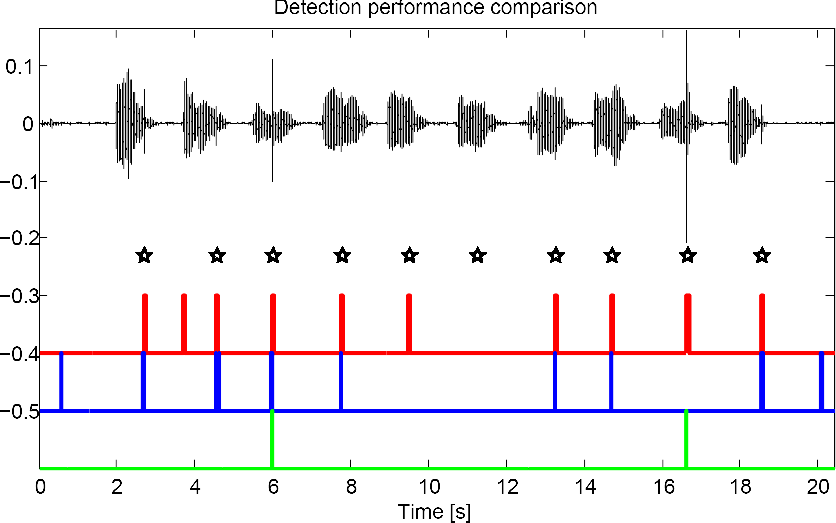
\includegraphics[width=12.5cm]{NBDetCompareLongTapsnTalk}}
%  \vspace{1.5cm}
  \centerline{(b) 10 taps embedded in 10 utterances. Stars indicate ground truth.}\medskip
\end{minipage}
\hfill
%
\caption{Detection results for sequences of taps.}
\label{fig:NBDetectionResults}
\end{figure}

\subsubsection{False detection rate}
To further quantify the performance of the algorithm a similar test to the above was run on 61 seconds of speech and 43 individual keyboards taps. The audio was recorded via an external microphone in 16kHz and all algorithms were tuned similarly to the previous test. The results of this test has been tabulated in Table~\ref{table:NBResultsTest}.

\begin{table}
\caption{Detection results}
\centering
\begin{tabular}{|l | c c c|}
\hline
                            & Noise Burst   & UKD       & Median        \\
 \hline
 Correct detection rate     & 34 \%         & 20 \%     & 50 \%         \\
 False detections pr second & 0             & 0.03      & 0.02          \\
 \hline
 \end{tabular}
 \label{table:NBResultsTest}
\end{table}

\subsection{AR Filter method results}
Figure~\ref{fig:ARFilterDetectionResults} shows, similar to Figure~\ref{fig:NBDetectionResults}, the detection performance for the AR filter method (red) in relation to that of the UKD\cite{Subramanya2007} (blue) and the standard median filter method (green). Figure~\ref{fig:ARFilterDetectionResults}(a) shows the algorithms performance on 10 clean keyboard strokes while Figure~\ref{fig:ARFilterDetectionResults}(b) shows an example of the algorithms' performance when the keyboard strokes are embedded in speech. As can be seen in Figure~\ref{fig:NBDetectionResults} with the proposed noise burst model, the AR filter model in Figure~\ref{fig:ARFilterDetectionResults} indicates a detection in between the first and the second correct detections. Both of these detections are clearly provoked by the sudden onset of the speech utterance and is considered a false detection.

\begin{figure}
\begin{minipage}[b]{1.0\linewidth}
  \centering
  \centerline{\includegraphics[width=12.5cm]{ARFiltCompareLongTaps.pdf}}
%  \vspace{2.0cm}
  \centerline{(a) 10 taps with no speech.}\medskip
\end{minipage}
%
\begin{minipage}[b]{1.0\linewidth}
  \centering
  \centerline{\includegraphics[width=12.5cm]{ARFiltCompareLongTapsnTalk.pdf}}
%  \vspace{1.5cm}
  \centerline{(b) 10 taps embedded in 10 utterances. Stars indicate ground truth.}\medskip
\end{minipage}
\hfill
%
\caption{Detection results for sequences of taps.}
\label{fig:ARFilterDetectionResults}
\end{figure}

Since the 3 detection methods compared in this section all work by thresholding some statistical value the maximum excitation for various signal types can be compared and ideally there should be a margin between correct detection and false detections in which a threshold limit can be set. Figures~\ref{fig:DetectPerfARFilt.pdf} - \ref{fig:DetectPerfMedian.pdf} are figures showing the maximum excitations for 40 different keystroke files and 53 different speech segments for the three different detection methods previously compared in this section. Figures~\ref{fig:DetectPerfARFilt.pdf} and \ref{fig:DetectPerfUKD.pdf} show that for both the AR filter and the UKD method, there is a distinct margin in between the lowest maximum excitation for a positive detection and the highest maximum detection for a false detection indicating that there are a range of values for which perfect detection could be achieved for this training set. The minimum response for correct detection is 1067 and 91.4 while the maximum response for a false detection, or for the clean speech segments, is 714.4 and 72.2 for the AR filter and UKD methods respectively. In relative terms the maximum response for a false detection in this test would be 67\% of the minimum correct detection response while the same number for the UKD method would be 79\%.
Figure~\ref{fig:DetectPerfMedian.pdf} shows that although the mean value for the maximum detection statistics are clearly separated, several samples give results within the range of 0.05, the lowest maximum detection for a keystroke, and 0.29, the highest maximum detection for a clean speech signal.

\begin{figure} %DetectPerfARFilt.pdf
\begin{minipage}[b]{1.0\linewidth}
  \centering
  \centerline{\includegraphics[width=12cm]{DetectPerfARFilt.pdf}
  \begin{picture}(0,0)
%\put(-310,275){a)}
%\put(-310,135){b)}
\end{picture}}
\end{minipage}
\caption{Maximum detector response for files with either a tap or some speech.}
\label{fig:DetectPerfARFilt.pdf}
\end{figure}

\begin{figure} %DetectPerfUKD.pdf
\begin{minipage}[b]{1.0\linewidth}
  \centering
  \centerline{\includegraphics[width=12cm]{DetectPerfUKD.pdf}
  \begin{picture}(0,0)
%\put(-310,275){a)}
%\put(-310,135){b)}
\end{picture}}
\end{minipage}
\caption{Maximum detector response for files with either a tap or some speech.}
\label{fig:DetectPerfUKD.pdf}
\end{figure}

\begin{figure} %DetectPerfMedian.pdf
\begin{minipage}[b]{1.0\linewidth}
  \centering
  \centerline{\includegraphics[width=12cm]{DetectPerfMedian.pdf}
  \begin{picture}(0,0)
%\put(-310,275){a)}
%\put(-310,135){b)}
\end{picture}}
\end{minipage}
\caption{Maximum detector response for files with either a tap or some speech.}
\label{fig:DetectPerfMedian.pdf}
\end{figure}

\subsubsection{False detection rate}

To evaluate the performance of any given detection algorithm the rate of false detections is often considered. Assuming that all positive detections were detected correctly, the false detection rate gives a measure of an algorithms sensitivity and therefore its performance.

In this comparison we will be comparing the Wavelet based detection algorithm, discussed in section~\ref{sec:WPdetection}, the STFT based UKD algorithm\cite{Subramanya2007} and a basic median based detection algorithm. Since all these detection algorithms investigated depend on various thresholds, it is important to construct a method for calibrating all methods so a valid comparison can be drawn. For this a set of 40 keyboard taps collected from a variety of sources was used. The threshold was set as the minimum value of the maximum responses of each tap for every model. In other words, the threshold was adjusted so that it would only just detect all 40 taps.

Figure~\ref{fig:maxes.pdf} shows the various maximum responses of each tap for all three detection methods. Had any of these methods produced a significantly lower response for only a few of the taps the calibration scheme chosen here would have put that detection method at a disadvantage. In this instance none of the methods produce significantly outlying responses. It is although noted that the Wavelet based detector does produce extremely high responses in some instances.

\begin{figure} %maxes.pdf
\centering
\includegraphics[width=120mm]{maxes.pdf}
\caption{Various detection algorithm response performance for the same 40 keystroke taps.}
\label{fig:maxes.pdf}
\end{figure}

Given the threshold set as described above, an additional 55 short audio segments (combined playing time of about 1 min) containing speech were analysed.

It was found that both the Wavelet and STFT based methods had 2 false detections while the median detector had 28 false detections. While the STFT UKD method might have identical performance to the Wavelet based method it should be noted that the UKD method requires a longer look-ahead and provides a coarser temporal resolution than the Wavelet based method.

\section{Discussion}\label{sec:WPdiscussion}
\subsection{Separation algorithm}

By visual inspection of Figures~\ref{fig:Separation_Residual_Example} through \ref{fig:SeparationWaveformExBig640.pdf} it is clear that the separation algorithm provides a reduction of speech while leaving transient noise events largely the same in the residual component. Audibly this effect is also clearly verified. Despite a distinct audible effect on the speech the tonal component alone manages a decreased maximum MSE from 5.2 to 3.2 as well as increasing the PSNR from 80.5 dB to 82 dB. While the maximum MSE is nearly halved in the tonal component of the signal, the original corruption site is still clearly visible in Figure~\ref{fig:SeparationError.pdf}. The original corruption is nearly inaudible in the tonal component and Figure~\ref{fig:SeparationErrorData.pdf} shows in more detail the waveform of the corruption site. The MSE might still be significant in Figure~\ref{fig:SeparationError.pdf} but Figure~\ref{fig:SeparationErrorData.pdf} reveals that this might mainly be due to phase shifts around the corruption site with am inaudible effect.

\subsection{Detection algorithms}
Two different, but related, detection algorithms have been presented in this chapter; the noise burst model algorithm and the AR filtering algorithm. These two have been compared to two other approaches; the UKD algorithm\cite{Subramanya2007} and a median filter algorithm. While the median filter algorithm provides a benchmark for one of the simplest approaches previously used for similar applications, the UKD algorithm represents the best alternative in the literature.

%Discussion of NBDetectionResults and NBResultsTest
It is clear from Figure~\ref{fig:NBDetectionResults} and Table~\ref{table:NBResultsTest} that both the Noise Burst and the UKD algorithm outperform the standard median filter approach. Figure~\ref{fig:NBDetectionResults}(a) shows the UKD algorithm being slightly more sensitive than the Noise Burst model, while in Figure~\ref{fig:NBDetectionResults}(b) the UKD appears slightly less sensitive to embedded taps while finding more false detections than the Noise Burst model. It is although worth noting that the keyboard strokes generally missed are the ones for which the impulse amplitude appears to not exceed that of the speech segment. For all methods tested this does appear to be a difficult detection scenario especially at low (for audio in general) sample rates of 16kHz. At higher sample rates, where the speech would take up a lower proportion of the bandwidth, the algorithms should perform better assuming that the noise pulse's spectrum is being limited by the current sample rate. Table~\ref{table:NBResultsTest} shows the Noise Burst algorithm being more sensitive than UKD while all tested algorithms maintain a low false detection rate. The median detector's good performance in the last test is probably explained by the relatively loud transients in the audio compared to the speech.

Figure~\ref{fig:NBDetCompare} specifically shows one of the strengths of the noise burst algorithm in relation to the UKD algorithm. While both algorithms catch elements of both keyboard strokes the UKD algorithm misses the initial impulse of the second keyboard stroke. Additionally the noise burst algorithm gives a clear estimate of the extent of the corruption. The detection rate results from Table~\ref{table:NBResultsTest} also shows similar results although again slightly in favour of the noise burst model.

In general the results presented in section~\ref{sec:WPdetectionNBresults} indicate that the noise burst model outperforms both the UKD and the median filter method. A significant issue with the noise burst model is although that it requires a good estimate for the variance of noise pulses for the algorithm to perform well in various scenarios which will have to be updated requiring additional algorithmic complexity. The results presented in this chapter has attempted to assess the algorithms on a variety of data but the amount of tuning required for the noise burst model to perform well does make a simple and general implementation infeasible.

The AR filter method was considerably easier to implement, more generally applicable and computationally simpler. Figure~\ref{fig:ARFilterDetectionResults} shows the results from a similar test to that of Figure~\ref{fig:NBDetCompare} with the AR filter method generally being more sensitive. While the AR filter method does appear to trigger more false detections, closer inspection of the underlying data does suggest that some of these are in fact secondary impulses while others are other spurious acoustic noise pulses. The only clearly falsely detected impulse is the detection of the sharp speech onset in the second speech segment. The same speech segment that the noise burst model falsely detected, as seen in Figure~\ref{fig:NBDetCompare}. As with the noise burst model the AR filter method also misses a detection although a different one in this case.

While the visible real world detection results, Figures~\ref{fig:ARFilterDetectionResults} and \ref{fig:NBDetCompare}, are informative, the problem of assessing objectively what qualifies as a false detection can be difficult. The Figures~\ref{fig:DetectPerfARFilt.pdf} - \ref{fig:DetectPerfMedian.pdf} provide clear representation of the range of excitation values for a set of 40 audio files with keyboard strokes and 53 files including speech and no noise pulses. The general margin between these two ranges indicate the robustness of the algorithm. It is seen from these plots the AR filter method, Figure~\ref{fig:DetectPerfARFilt.pdf}, and the UKD algorithm, Figure~\ref{fig:DetectPerfUKD.pdf}, clearly outperforms the median filter approach, Figure~\ref{fig:DetectPerfMedian.pdf}, which shows a significant overlap of the two ranges. While the AR filter approach has maximum responses with higher variance the UKD algorithm has a more consistent response. The lower variance of the UKD response is probably due to a smoothing effect by the larger size of the Fourier transform windows used in this procedure, since both method respond to similar wide band noise characteristics in the impulses. The two methods also have responses on very different scales so a direct comparison can be difficult but based on the relationship between the minimum response for a positive detection and the maximum response for a false detection the AR filter method provides an increased margin and thereby robustness. Other practical concerns speak in favour of the AR filter method as well. The AR filter method also provides provides higher temporal resolution, via the Wavelet Transform, than the UKD algorithm in addition to not requiring the additional look-ahead. Better temporal resolution provides more accurate detection and therefore more accurate restoration. Less required look-ahead in the algorithm makes real time implementations more feasible and reduces in-built latency. 

%Although the algorithms generally performed well on the data sampled at 16kHz in this section, which is common in wide band VoIP applications, it should be noted that for audio recorded at higher sample rates the
%narrowband telecommunication systems work against these detection algorithms by having a less sparse spectrum.
\section{Conclusions}\label{sec:WPconclusions}

This chapter has explored a variety of noise impulse detectors for the express purpose of detecting keyboard strokes for a real time communication system. The impulses created by the keyboard stroke was found to generally consist of a number of noise pulses each associated with various mechanical interactions with the keyboard itself. All of these pulses had varying amplitudes and timing in relation to each other depending on the a range of parameters. The individual detection of these different pulses appears to be the only feasible approach to the detection step due to this variability. Two detectors were developed and tested in this section; the noise burst model and the AR filter method. These were compared and contrasted with a state of the art algorithm for this purpose, the UKD algorithm\cite{Subramanya2007}, and a basic and largely legacy approach using a median filter.

Tests suggested that with careful tuning the noise burst model performed at least as well as the UKD algorithm on the data sets used, while providing additional functionality. It was although also noted that the algorithm was reliant on a variety of parameters that complicated the application of the algorithm and could limit the general applicability of the algorithm.

While it is difficult to conclusively state, based on the results in section~\ref{sec:WPresults}, that the AR filter method is superior to the noise burst model and the UKD algorithm, considering practical implementation concerns it provides a detection performance at least on par with the competition without the in-built latency and poor temporal resolution of the UKD algorithm or the required training and complexity of the noise burst model. Predictably, all algorithms tested outperformed the median filter algorithm. 
% ------------------------------------------------------------------------


%%% Local Variables:
%%% mode: latex
%%% TeX-master: "../thesis"
%%% End: \  %Detection
%\chapter{Transient Noise Restoration}\label{ch:TransientNoiseRestoration}

\ifpdf
    \graphicspath{{Chapter6_TransNoiseRest/Chapter6Figs/PNG/}{Chapter6_TransNoiseRest/Chapter6Figs/PDF/}{Chapter6_TransNoiseRest/Chapter6Figs/}{Chapter6_TransNoiseRest/Chapter6Figs/Subjective/}{Chapter6_TransNoiseRest/Chapter6Figs/Results/}}
\else
    \graphicspath{{Chapter6_TransNoiseRest/Chapter6Figs/EPS/}{Chapter6_TransNoiseRest/Chapter6Figs/}}
\fi

As mentioned previously, the keyboard stroke removal algorithm can roughly be divided into two. Chapter~\ref{ch:TransientNoiseDetection} dealt with the task of detecting keyboard stroke noise and calculating the corruptions extent. Based on analysis of the data it was also concluded that while a model based approach could perform well on isolated keyboard stroke examples tuning it for more general cases would be difficult. This chapter will explore the second, and final step, of the keyboard stroke removal system and focus on the restoration of the corrupted samples of the audio sequence. While the complete removal of all localised transient noise is the ultimate goal of this chapter, any significant reduction in audibility or subjective nuisance will also be acceptable. To evaluate this goal this chapter will also include a subject study of the restoration quality.

In this chapter a variety of methods will be explored. While the preferred detection algorithm from Chapter~\ref{ch:TransientNoiseDetection} was the AR filter method, the noise burst model lent itself to an interesting restoration model based on the noise burst assumption, which will also be explored in this chapter.

\section{Residual Restoration}
Based on the pre processing stage from Equation~\ref{eq:modelgeneral} the restoration section is separated into two major sections. Firstly the restoration or interpolation of the corrupted samples from the residual component of the signal will be explored. This sparse signal of transient components from the audio was found to contain a majority of the initial impulse of the keyboard strokes.

The second part of this section will focus on restoring and removing spurious tonal components caused by the keyboard stroke. Certain keyboard types in particular were found to produce noise pulses with more tonal components than others, and in particular loud strokes on the keyboard were also found to exacerbate this issue. The methods developed in this part of the chapter will largely be of a heuristic nature.

The restoration of the sparse residual component can be formulated as follows. In this chapter the detection state is presumed known and will be treated as a binary vector $\boldsymbol{i}$ containing a high value $i_t = 1$ for a detection and a low value $i_t = 0$ for no detection. Consider an audio segment $\boldsymbol{x}$ of length $N$ with a corrupted section starting at sample $m$ and of length $l$. The corrupted sequence can now be described as 3 separate sections with the unknown section being $\boldsymbol{x_{(i)}} = [x_m,x_{m+1},\ldots,x_{m+l-1}]$, the known section before and after the corruption respectively $\boldsymbol{x}_{\boldsymbol{-(i)}a} = [x_1,x_{2},\ldots,x_{m-1}]$ and $\boldsymbol{x}_{\boldsymbol{-(i)}b} = [x_{m+1},x_{m+2},\ldots,x_{N}]$. The total sequence is therefore

\begin{equation}\label{eq:RestBasicModel}
\boldsymbol{x} = \left[ \boldsymbol{x}_{\boldsymbol{-(i)}a}\quad\boldsymbol{x_{(i)}}\quad\boldsymbol{x}_{\boldsymbol{-(i)}b} \right].
\end{equation}


\subsection{Noise insertion}
The simplest restoration algorithm proposed in this chapter features a simple method for replacing corrupted samples with random noise.

Consider the wavelet coefficients from a decomposition following the detection stage. Similar to equation~\ref{eq:RestBasicModel} we have for the wavelet coefficients that

\begin{equation}\label{eq:RestBasicModelWavelet1}
\boldsymbol{X_j} = \left[ \boldsymbol{X}_{\boldsymbol{j,-(i)}a}\quad\boldsymbol{X}_{j,\boldsymbol{(i)}}\quad\boldsymbol{X}_{j,\boldsymbol{-(i)}b} \right],
\end{equation}
for $\boldsymbol{X_j}$ the $j$th terminal node, $j \in \{1, \ldots, J\}$.

The samples to replace are drawn from a zero-mean Gaussian distribution with the same variance $\sigma^2_{j,a}$ as the preceding segment $\boldsymbol{X}_{\boldsymbol{j,-(i)}a}$.

\begin{equation}\label{eq:RestNoiseInsertionModelVariance1}
\boldsymbol{X}_{j,\boldsymbol{(i)}} \sim \mathcal{N}\left(0, \sigma^2_{j,a} \right).
\end{equation}

If data is available following a corruption, the variance $\sigma^2_{j,b}$ of the succeeding segment $\boldsymbol{X}_{\boldsymbol{j,-(i)}b}$ can be used in a similar fashion. Too facilitate a smooth transition a cross fading between the two random signals should be implemented.

Figure~\ref{fig:ResultsNoiseInsertion.pdf} shows an example of the restoration process described above. Figure~\ref{fig:ResultsNoiseInsertion.pdf}(a) shows a set of the initial wavelet coefficients for a keystroke. The corrupted region has been removed in Figure~\ref{fig:ResultsNoiseInsertion.pdf}(b) and replaced with zero-mean Gaussian noise with the red plot showing noise generated from the segment preceding the corruption and the red blue plot showing noise generated from the segment succeeding it. The two signals have been windowed and the final segment will be the addition of the two noise segments.

\begin{figure} %ResultsNoiseInsertion.pdf
\centering
\includegraphics[width=110mm]{ResultsNoiseInsertion.pdf}
\begin{picture}(0,0)
\put(-300,390){(a)}
\put(-300,180){(b)}
\end{picture}
\caption{Example of noise insertion algorithm. (a) Original corrupted signal, (b) Forward (red) and backward (blue) noise interpolation.}
\label{fig:ResultsNoiseInsertion.pdf}
\end{figure}

\subsection{Forwards and backwards FIR filtering}
%Model theory
A simple approach to restoration of short corrupted intervals is to replace the corrupted samples and filter the corrupted region with an FIR filter with parameters drawn from the segment immediately prior to $\boldsymbol{x}_{\boldsymbol{-(i)}a}$ and following $\boldsymbol{x}_{\boldsymbol{-(i)}b}$ (if available) the corruption.

Consider first the block of data samples $\boldsymbol{x}$ drawn from an AR process with parameters $\boldsymbol{a}$. Given a known estimate of the detection state $\boldsymbol{i}$, zero pad the corrupted samples.

\begin{equation}\label{eq:RestBasicModelFilterZeros}
\boldsymbol{x} = \left[ \boldsymbol{x}_{\boldsymbol{-(i)}a}\quad \left[0,\ldots,0\right] \quad\boldsymbol{x}_{\boldsymbol{-(i)}b} \right].
\end{equation}

The block of data $\boldsymbol{x}$ is then filtered using the AR parameters up until the end of the corrupted section,

\begin{equation}\label{eq:RestBasicModelFilterEQ}
\boldsymbol{\hat{x}}_f = \Sigma_p^P \boldsymbol{x}_{n-p}a_p.
\end{equation}

The output signal $\boldsymbol{\hat{x}}_f$ now contains a basic estimate of the corrupted section which will be called the forward filtered estimate. Reversing the order of the samples in $\boldsymbol{x}$ denoting it $\boldsymbol{x'}$ and applying the filtering step up to the end of the zeroed out corruption section gives an estimate for the backwards filtered estimate.

\begin{equation}\label{eq:RestBasicModelFilterEQR}
\boldsymbol{\hat{x}'}_b = \Sigma_p^P \boldsymbol{x'}_{n-p}a_p.
\end{equation}

The forward $\boldsymbol{\hat{x}}_f$ and backward $\boldsymbol{\hat{x}}_b$ filtered estimates can now, if both are available, be faded together to produce a combined estimate for the corrupted sequence $\boldsymbol{\hat{x}}$.

An example of a reconstructed section on can be seen in Figure~\ref{fig:ResultsFiltering.pdf}. It is noted that for this example the reconstruction is done on wavelet coefficients. Figure~\ref{fig:ResultsFiltering.pdf}(a) shows, as in Figure~\ref{fig:ResultsNoiseInsertion.pdf}, the original signal and Figure~\ref{fig:ResultsFiltering.pdf}(a) shows an example of the various parts of the reconstruction.

\begin{figure} %ResultsFiltering.pdf
\centering
\includegraphics[width=110mm]{ResultsFiltering.pdf}
\begin{picture}(0,0)
\put(-300,390){(a)}
\put(-300,180){(b)}
\end{picture}
\caption{Example of forwards backwards algorithm. (a) Original corrupted signal, (b) Forward (red) and backward (blue) filtering interpolation.}
\label{fig:ResultsFiltering.pdf}
\end{figure}

\subsubsection{Filtering with noise}
It is possible to combine the noise insertion algorithm with the forward backward filtering algorithm to avoid a clearly audible dip in the loudness. This method proceeds as the original noise insertion method after which the forward backward filtering step is performed without zeroing the corrupted region.

Figure~\ref{fig:ResultsNoiseInsertionFiltering.pdf} shows an example of the noise insertion and filtering method applied to the same restoration example as in Figure~\ref{fig:ResultsNoiseInsertion.pdf} and \ref{fig:ResultsFiltering.pdf}.

\begin{figure} %ResultsNoiseInsertionFiltering.pdf
\centering
\includegraphics[width=110mm]{ResultsNoiseInsertionFiltering.pdf}
\begin{picture}(0,0)
\end{picture}
\caption{Example of forwards backwards algorithm.}
\label{fig:ResultsNoiseInsertionFiltering.pdf}
\end{figure}

\subsection{Burst scaling}
A different restoration approach can be derived from the noise burst detection method proposed in section~\ref{sec:WPdetectionNB}.
Based on the separation of the original data sequence in Equation~\ref{eq:modelgeneral} it was assumed that the majority of the transient information will be located in the residual, or non-tonal component. Considering the detection methods employed on the residual component, the restoration process could be done in either the time or the wavelet domain $w(n)$.

A Bayesian approach proceeds by estimating $p(\boldsymbol{v}_n | \boldsymbol{w}_n, i_n)$. Using Bayes' rule we get that

\begin{equation}\label{eq:BayesInterp}
p(\boldsymbol{v}_n | \boldsymbol{w}_n, i_n) \propto p(\boldsymbol{w}_n | \boldsymbol{v}_n , i_n) p(\boldsymbol{v}_n | i_n),
\end{equation}
where
\begin{equation}\label{eq:w|vi}
p(\boldsymbol{w}_n | \boldsymbol{v}_n, i_n = 1) = \mathcal{N}(\boldsymbol{v}_n, \Lambda),
\end{equation}
and
\begin{equation}\label{eq:v2}
p(\boldsymbol{v}_n | i_n) = p(\boldsymbol{v}_n) = \mathcal{N}(0, C_v).
\end{equation}
Substituting equation (\ref{eq:w|vi}) and (\ref{eq:v2}) into equation (\ref{eq:BayesInterp}) where the product is proportional to a third Gaussian,
\begin{equation}\label{eq:vwi}
p(v_n | \boldsymbol{w}_n, i_n = 1) \propto \mathcal{N}\left({(C_v + \Lambda)^{-1} C_v\boldsymbol{w}_n}, (C_v^{-1} + \Lambda^{-1})^{-1}\right)
\end{equation}

%\frac{\boldsymbol{w}_n}{\Lambda}\right).
In this case where both the background noise $v_n$ and the noise burst $\theta_n$ are Gaussian, estimating the mean of the conditional distribution equates to simply scaling corrupted samples by a factor of $({C_v + \Lambda})^{-1}{C_v}$ in a Wiener-style wavelet shrinkage (note the simple form of this in our case with diagonal covariance matrices).

An example of the burst scaling algorithm is seen in Figure~\ref{fig:ResultsScaled.pdf}. The reference variance for the wavelet coefficient sets $C_v$ is taken over a 5 second sequence. The pulse variance $\Lambda$ is a trained value which might vary from session to session, but for the restoration stage here the first 150 samples of the detected impulse is used.

\begin{figure} %ResultsScaled.pdf
\centering
\includegraphics[width=100mm]{ResultsScaled.pdf}
\begin{picture}(0,0)
%\put(-245,235){Restored Example}
%\put(-200,0){Time}
\end{picture}
\caption{Examples of the burst scaling algorithm restoring corrupted wavelet coefficients.}
\label{fig:ResultsScaled.pdf}
\end{figure}

%While assuming corruptions as noise bursts works well for detection, it was found that a more pleasing restoration was achieved by simply inserting white noise bursts with background variance in the corrupted regions. Figure~\ref{fig:compareRecon} shows an example of the restoration on the example result from Figure~\ref{fig:Separation_Residual_Example} An even simpler restoration approach could potentially entirely remove the offending coefficients and a more complicated approach attempt to fill in the corrupted coefficients with an AR process trained on preceding and succeeding coefficients. Having estimated the most likely state of $i_n$ it is sometimes necessary also to filter out any very low frequency components of the transient that were removed with the voiced speech. Figure~\ref{fig:compareRecon} shows an example of the restored signal with the corrupted regions filtered with a high pass filter with a cutoff frequency of 120 Hz.
%
%\begin{figure} %compareRecon.pdf
%\centering
%\includegraphics[width=100mm]{compareRecon.pdf}
%\begin{picture}(0,0)
%%\put(-245,235){Restored Example}
%%\put(-200,0){Time}
%\end{picture}
%\caption{Example of the algorithm interpolating corrupted waveform samples.}
%\label{fig:compareRecon}
%\end{figure}
%
%The final stage of the algorithm proceeds by recombining the processed residual with the keystrokes removed and the dictionary of tonal components from equation~\ref{eq:modelgeneral}.
%
%%Standard restoration, interpolation


\subsection{Least Squares AR (LSAR)}\label{sec:ResidualRestorationLSAR}
For the restoration of samples in the residual component the Least Squares AR (LSAR) interpolator is considered here\cite{Godsill1998book}.

Assuming that the residual coefficients $\mathbf{x}$ are drawn from an AR process with parameters $\mathbf{a}$, and where

\begin{equation}\label{eq:LSAR0} \mathbf{A} =
\begin{bmatrix}
    -a_P    & \ldots & -a_1 & 1 & 0 & 0 & \ldots & 0 & 0 \\
    0       & -a_P & \ldots & -a_1 & 1 & 0 & 0 & \ldots & 0 \\
    \vdots  & \vdots    & \ddots & \ddots & \ddots & \ddots & \ddots & \vdots & \vdots \\
    \ldots  & 0 & 0 & -a_P    & \ldots & -a_1 & 1 & 0 & 0 \\
    0       & \ldots  & 0 & 0 & -a_P    & \ldots & -a_1 & 1 & 0 \\
    0       & 0 & \ldots  & 0 & 0 & -a_P    & \ldots & -a_1 & 1 \\
\end{bmatrix}.
\end{equation}

The excitation vector $\mathbf{e}$ can be expressed as

\begin{equation}\label{eq:LSAR1}
  \mathbf{e} = \mathbf{A}\mathbf{x},
\end{equation}

where $\mathbf{X}$, the data vector, can be reexpressed in terms of corrupted and uncorrupted, or known $\mathbf{K}$ and unknown $\mathbf{U}$), samples

\begin{align}\label{eq:LSAR2}
  \mathbf{e} = & \mathbf{A} (\mathbf{U}\mathbf{x}_{\mathbf{(i)}} + \mathbf{K}\mathbf{x}_{\mathbf{-(i)}}) \\
  \mathbf{e} = & \mathbf{A}_{\mathbf{(i)}} \mathbf{x}_{\mathbf{(i)}} + \mathbf{A}_{\mathbf{-(i)}}\mathbf{x}_{\mathbf{-(i)}}.
\end{align}

Now the sum squared prediction error can be calculated as

\begin{equation}\label{eq:LSAR3}
  E = \sum^N_{n=P+1} e^2_n = \mathbf{e}^T\mathbf{e}.
\end{equation}

The Least Squares (LS) interpolator is obtained as the interpolated data vector $\mathbf{x}_{\mathbf{(i)}}$ which minimises the error in equation~\ref{eq:LSAR3}:

\begin{equation}\label{eq:LSAR4}
  \mathbf{x}^{\mathrm{LS}}_{\mathbf{(i)}} = \argmin{\mathbf{x}_{\mathbf{(i)}}} \{ E \}.
\end{equation}

$E$ can expanded and differentiated to find its minimum:

\begin{align}\label{eq:LSAR5}
  E = & \mathbf{e}^T\mathbf{e} \\
  \frac{\partial E}{\partial \mathbf{x}_{\mathbf{(i)}}} = & 2\mathbf{e}^T \frac{\partial \mathbf{e}}{\partial \mathbf{x}_{\mathbf{(i)}}} \\
   = & 2 (\mathbf{A}_{\mathbf{(i)}} \mathbf{x}_{\mathbf{(i)}} + \mathbf{A}_{\mathbf{-(i)}}\mathbf{x}_{\mathbf{-(i)}})^T \mathbf{A}_{\mathbf{(i)}} = 0
\end{align}

Solving for $\mathbf{x}_{\mathbf{(i)}}$ we have that:

\begin{equation}\label{eq:LSAR6}
  \mathbf{x}^{\mathrm{LS}}_{\mathbf{(i)}} = - (\mathbf{A}_{\mathbf{(i)}}^T \mathbf{A}_{\mathbf{(i)}} )^{-1}\mathbf{A}_{\mathbf{(i)}}^T\mathbf{A}_{\mathbf{-(i)}}\mathbf{x}_{\mathbf{-(i)}}
\end{equation}

An example of the LSAR interpolation algorithm is shown in Figure~\ref{fig:RestoredLSARExample}(a) and \ref{fig:RestoredLSARExample2}(b), where 2 different sets of Wavelet coefficients have had an impulse detection restored. Both examples are of audio sampled at 16kHz and coefficients are from a Wavelet decomposition done to the third level. Figure~\ref{fig:RestoredLSARExample}(a) uses the same detection example as the previous examples while  Figure~\ref{fig:RestoredLSARExample2}(b) shows a restoration example, from the same audio sequence, which showcases more of the algorithms restoration abilities.

\begin{figure}
\begin{minipage}[b]{1.0\linewidth}
  \centering
  \centerline{\includegraphics[width=10cm]{RestoredLSARExample1.pdf}}
%  \vspace{2.0cm}
  %\centerline{(a)}\medskip
\end{minipage}
\begin{minipage}[b]{1.0\linewidth}
  \centering
  \centerline{\includegraphics[width=10cm]{RestoredLSARExample2.pdf}}
  \begin{picture}(0,0)
\put(-120,382){a)}
\put(-120,195){b)}
\end{picture}
%  \vspace{1.5cm}
  %\centerline{(b)}\medskip
\end{minipage}
\caption{Examples of the LSAR algorithm interpolating corrupted wavelet coefficients.}
\label{fig:RestoredLSARExample}
\end{figure}

%\begin{figure}% %Restore_LSAR_1.pdf
%\centering
%\includegraphics[width=100mm]{Restore_LSAR_1.pdf}
%\begin{picture}(0,0)
%\put(-245,235){Restored Wavelet coefficients Example 1}
%%\put(-200,0){Time}
%\end{picture}
%\caption{Example of the LSAR algorithm interpolating 85 missing Wavelet coefficients at level 3.}
%\label{fig:Restore_LSAR_1.pdf}
%\end{figure}
%
%\begin{figure} %Restore_LSAR_2.pdf
%\centering
%\includegraphics[width=100mm]{Restore_LSAR_2.pdf}
%\begin{picture}(0,0)
%\put(-245,235){Restored Wavelet coefficients Example 2}
%%\put(-200,0){Time}
%\end{picture}
%\caption{Example of the LSAR algorithm interpolating 85 missing Wavelet coefficients at level 3.}
%\label{fig:Restore_LSAR_2.pdf}
%\end{figure}

\section{Tonal Restoration}
While the aim of the pre processing separation stage is to separate out tonal components from transient noise events, the tonal components themselves occasionally retain components introduced by the noise events. These tonal noise components are not always present, but factors such as the amplitude of the impulse, mechanical properties of the keyboard or the laptop enclosure and even the surface on which the keyboard or computer is placed can have an impact on whether or not these components are present to the extent that get identified as tonal components. Constraints such as frame sizes in the system can also add to the amount of noise leaking through to the tonal components. A short frame size can contribute to this effect.

\subsection{Basic filtering}\label{sec:TonalFiltering}
The most common noise component left in the tonal component of the signal is a low frequency \emph{bump}. Figure~\ref{fig:TonalArtefactSpectrumExample.png} shows an example of this, with an accompanying spectrogram. While it may be difficult to clearly visualise the extent of the corruption within a speech segment, it is although clearly audible.\footnote{\sound{Tonal\_Example.wav}} 

\begin{figure} %TonalArtefactSpectrumExample.png
\centering
\includegraphics[width=120mm]{TonalArtefactSpectrumExample.png}
\begin{picture}(0,0)
%\put(-320,442){a)}
%\put(-320,290){b)}
%\put(-320,140){c)}
\end{picture}
\caption{Example of low frequency tonal noise. A \emph{bump}. Top: Waveform and Bottom: Spectrogram of same sequence.}
\label{fig:TonalArtefactSpectrumExample.png}
\end{figure}

A simple approach to removing low frequency noise is to apply standard high pass filter to the corrupted region. Fading in and out from this filtered segment will remove the effect of discontinuities. Figure~\ref{fig:TonalFilteringExample.pdf} shows the same example of a tonal noise component as in Figure~\ref{fig:TonalArtefactSpectrumExample.png} and the process for removing it. In Figure~\ref{fig:TonalFilteringExample.pdf}(a) the original corrupted signal can be seen together with a plot of the detection state. The unrestored tonal component is seen in Figure~\ref{fig:TonalFilteringExample.pdf}(c) with a mixing indicator showing the state of the mixing process which tapers the amplitude from 100\% to 0\% in 200 samples or an $1/80$ of a second at the sampling rate of 16000 Hz. Figure~\ref{fig:TonalFilteringExample.pdf}(b) shows the inverse mixing indicator and the high pass filtered signal with a cutoff frequency of 120 Hz. 

\begin{figure} %TonalFilteringExample.pdf
\centering
\includegraphics[width=120mm]{TonalFilteringExample.pdf}
\begin{picture}(0,0)
\put(-320,442){a)}
\put(-320,290){b)}
\put(-320,140){c)}
\end{picture}
\caption{Example of simple tonal restoration using filtering. a) Original complete signal and detection state, b) High pass filtered (200Hz) tonal component with mixing indicator, and c) original tonal component with mixing indicator.}
\label{fig:TonalFilteringExample.pdf}
\end{figure}


\subsection{Historic filtering}
%- Historic Frequency logic and filtering (amplitudes)
%- Future restoration (fading)
While the separation algorithm works by modeling the speech as distinctive tonal components some keystroke noise pulses also exhibit strong tonal components beyond those seen in section~\ref{sec:TonalFiltering}. As mentioned previously, this may be due to a range of physical conditions but possibly also due to constraints on the frame size in a system. In this section a frame size of 10 ms is assumed. 

Figure~\ref{fig:TonalRestoration_Spec_Orig.png} shows the spectrogram of a keyboard noise pulse embedded in a voiced audio segment. The method described here will be applied to this audio example and followed throughout this section.

\begin{figure} %TonalRestoration_Spec_Orig.png
\centering
\includegraphics[width=100mm]{TonalRestoration_Spec_Orig.png}
\begin{picture}(0,0)
\put(-200,235){Spectrum of original signal}
%\put(-200,0){Time}
\end{picture}
\caption{Example of corrupted audio segment.}
\label{fig:TonalRestoration_Spec_Orig.png}
\end{figure}

Figure~\ref{fig:TonalRestoration_Spec_ResidualRestoration.png} shows a spectrogram of the audio segment from Figure~\ref{fig:TonalRestoration_Spec_Orig.png} with the LSAR residual restoration from section~\ref{sec:ResidualRestorationLSAR} applied. The separation algorithm has largely kept the voiced signal below 1500 Hz intact but some higher frequency information from the noise pulse has also been detected as tonal components and hence are still clearly visible in the spectrogram. These components, combined with the underlying voiced signal, is what can sometimes be seen detected as tonal components by the separation algorithm. Rather that replacing the data from the influenced buffers completely, like was done for the majority of the residual restoration algorithms, this sections will explore a heuristic method for filtering out interfering tonal components while keeping voiced components intact and undisturbed.

\begin{figure} %TonalRestoration_Spec_ResidualRestoration.png
\centering
\includegraphics[width=100mm]{TonalRestoration_Spec_ResidualRestoration.png}
\begin{picture}(0,0)
\put(-245,235){Spectrogram of signal after residual restoration}
%\put(-200,0){Time}
\end{picture}
\caption{Example of residual restored audio segment}
\label{fig:TonalRestoration_Spec_ResidualRestoration.png}
\end{figure}

Since voiced components of speech generally are seen for at least 100 ms, this tonal restoration algorithm starts by keeping a record of active tonal atoms. These are already computed through the separation algorithm and so this only requires additional memory while running. Figure~\ref{fig:TonalRestoration_Spec_ResidualRestorationFrames.png} shows a grid of 10 ms frames overlayed on the previous audio frames. The grid in Figure~\ref{fig:TonalRestoration_Spec_ResidualRestorationFrames.png} indicates the extent of historic buffer and the data stored will be the tonal components that are selected by the separation algorithm as well as the magnitude of these frequencies within the buffers.

\begin{figure} %TonalRestoration_Spec_ResidualRestorationFrames.png
\centering
\includegraphics[width=100mm]{TonalRestoration_Spec_ResidualRestorationFrames.png}
\begin{picture}(0,0)
\put(-250,235){Spectrogram of signal after residual restoration}
%\put(-200,0){Time}
\end{picture}
\caption{Example of tonal filtering algorithm of the data from Figure~\ref{fig:TonalRestoration_Spec_Orig.png}}
\label{fig:TonalRestoration_Spec_ResidualRestorationFrames.png}
\end{figure}

Figure~\ref{fig:TonalRestoratio_FramesLogic.pdf} shows a diagram of the logic in the tonal filtering algorithm applied to the tonal component of a frame or buffer that is found to be corrupted by a noise pulse. The algorithm proceed by calculating the binary sum vector from the magnitude history buffer. This vector will serve as a template for which frequencies would be expected in a corrupted frame. The vector in Figure~\ref{fig:TonalRestoratio_FramesLogic.pdf} annotated as ``Noise profile'' indicates tonal components detected during the corrupted frame. Filtering the current noise profile based on the magnitude history it is now possible to remove newly introduced frequencies that likely are due to the corruption.

\begin{figure} %TonalRestoratio_FramesLogic.pdf
\centering
\includegraphics[width=120mm]{TonalRestoratio_FramesLogic.pdf}
\begin{picture}(0,0)
\put(-260,265){Tonal filtering algorithm diagram}
\put(-340,25){Magnitude}
\put(-340,10){history}

\put(-240,25){Binary}
\put(-240,10){sum}

\put(-130,25){Noise}
\put(-130,10){profile}

\put(-25,25){Filtered}
\put(-25,10){noise frame}
\end{picture}
\caption{Example of part of the tonal restoration algorithm.}
\label{fig:TonalRestoratio_FramesLogic.pdf}
\end{figure}

While the filtered tonal components in a corrupted frame might now contain only plausibly correct tonal components these might still be of a significantly higher magnitude that seen in the previous uncorrupted voiced speech frames. Figure~\ref{fig:TonalRestoratio_FramesLogic2.pdf} shows a diagram of how the tonal restoration algorithm proceeds by scaling the filtered tonal components to a plausible magnitude. The median values from the historic magnitude buffer is computed and applied to the filtered tonal components.

\begin{figure} %TonalRestoratio_FramesLogic2.pdf
\centering
\includegraphics[width=100mm]{TonalRestoratio_FramesLogic2.pdf}
\begin{picture}(0,0)
\put(-250,265){Tonal scaling algorithm diagram}
\put(-280,20){Magnitude}
\put(-280,5){history}

\put(-180,20){Median}
\put(-180,5){values}

\put(-110,20){Filtered}
\put(-110,5){noise frame}

\put(-20,20){Filtered + scaled}
\put(-20,5){noise frame}
\end{picture}
\caption{Example of part of the tonal restoration algorithm.}
\label{fig:TonalRestoratio_FramesLogic2.pdf}
\end{figure}



\begin{figure} %TonalRestoratio_Spec_MagFiltScale.png
\centering
\includegraphics[width=100mm]{TonalRestoratio_Spec_MagFiltScale.png}
\begin{picture}(0,0)
\put(-250,235){Spectrum of signal after residual restoration}
\end{picture}
\caption{Example of residual restored and magnitude scaled audio segment}
\label{fig:TonalRestoratio_Spec_MagFiltScale.png}
\end{figure}

After applying both tonal filtering and rescaling Figure~\ref{fig:TonalRestoratio_Spec_MagFiltScale.png} shows the resulting spectrogram. While the initial pulse has been removed from the spectrogram a secondary pulse is still visible. This pulse shows how louder pulses will influence multiple buffers and hence it is necessary to employ filtering procedures for a number of frames after each detected corruption.

Figure~\ref{fig:TonalRestoratio_TonalFuture.pdf} shows a diagram of the logic employed to filter out remnants of noise pulses following a keyboard stroke detection. The algorithm contains 2 major components. First it applies a window function to the future tonal components so at the end of the procedure the algorithm performs as before a corruption was seen. Secondly the algorithm continues to apply the filtering and rescaling functions from the historic buffer. Since this second part of the algorithm is largely made up data this will be faded out as the real current data is faded back in.

\begin{figure} %TonalRestoratio_TonalFuture.pdf
\centering
\includegraphics[width=70mm]{TonalRestoratio_TonalFuture.pdf}
\begin{picture}(0,0)
%top
\put(-200,525){Tonal restoration of future buffers}

%left side
\put(-260,150){Magnitude}
\put(-260,135){history}

%right side
\put(10,440){Tonal}
\put(10,425){future}

\put(10,310){Fade in}
\put(10,20){Fade out}

\put(10,150){Filtered}
\put(10,135){future tones}
\end{picture}
\caption{Example of tonal restoration algorithm following a corruption.}
\label{fig:TonalRestoratio_TonalFuture.pdf}
\end{figure}

The effect of this complete tonal restoration algorithm can be seen in Figure~\ref{fig:TonalRestoratio_Spec_FullRestoration.png}. The corruption has been completely removed and replaced with plausible looking data.

\begin{figure} %TonalRestoratio_Spec_FullRestoration.png
\centering
\includegraphics[width=100mm]{TonalRestoratio_Spec_FullRestoration.png}
\begin{picture}(0,0)
\put(-240,235){Spectrogram of signal after full restoration}
\end{picture}
\caption{Example spectrogram of full restoration of audio segment.}
\label{fig:TonalRestoratio_Spec_FullRestoration.png}
\end{figure}

\section{Algorithm statement}
Figure~\ref{fig:restorationPP.pdf} shows a diagrammatic representation of the restoration stage of the algorithm. The restoration stage takes, as an input, $\boldsymbol{w}$ the wavelet packet coefficients, $\boldsymbol{i}$ the detection state and the tonal components. The restoration algorithms take as an input the relevant data to be restored as well as the detection state from the detection algorithm. The restored wavelet packet coefficients $\hat{\boldsymbol{w}}$ are passed through the inverse wavelet packet decomposition algorithm (IWPD) to restore the residual waveform before being combined with the restored tonal component to reconstruct the original restored signal $\hat{x}(n)$.

\begin{figure}%restorationPP.pdf
\centering
\includegraphics[width=120mm]{restorationPP.pdf}
\begin{picture}(0,0)
%line labels
\put(-330,145){$\boldsymbol{w}$}
\put(-175,130){$\hat{\boldsymbol{w}}$}
\put(-330,80){$\boldsymbol{i}$}
\put(-25,82){$\hat{x}(n)$}
\put(-340,35){Tonal}
\put(-340,20){components}


%box labels
\put(-252,30){Tonal}
\put(-252,15){restoration}
\put(-252,130){Residual}
\put(-252,115){restoration}
\put(-135,120){IWPD}
\end{picture}
\caption{Block diagram showing the general set up of the restoration algorithm.}
\label{fig:restorationPP.pdf}
\end{figure}

\section{Methods}
\subsection{Subjective test}
A subjective listening test was designed to gauge the preference of listeners to reconstructed corruptions in relation to the original corruption. Since the reconstruction procedure, in most cases, still leaves or introduces artifacts in the audio stream the experiment was intended to measure if the artificial noise would in fact be more of an audible nuisance than the original keystrokes.

Subjects were presented with 12 test sets consisting of 2 audio segments each; the original audio segment containing speech and a number of keystrokes and the reconstructed segment. The order of the original segment and the reconstructed segment was randomized throughout the trial. The audio segments used for this test was a mix of fast typing and slow typing, recorded through laptops and external microphones, naturally corrupted segments and keystrokes added to clean segments, male or female speech and a variety of keyboards types and makes.

The Graphical User Interface (GUI) presented to the test subjects is shown here in Figure~\ref{fig:SubjectiveExp_GUI.png}.

Subjects were asked to choose their preferred audio segment or the one they found the least annoying. If they found both segments equally annoying or equally pleasing they could opt to tick both boxes and proceed. All audio segments were sampled at 16kHz, ranged from 1 to 10 seconds in length (mainly in the range 3-5 seconds), and were run through a completely sequential version of the final algorithm as it would work implemented in a communication framework. All subjects used the same set of AKG K-240 M1 circumaural open back headphones in a quiet office environment through a laptop computer audio interface and were allowed to replay audio segments as they pleased. The test was conducted on 16 individuals found in and around the office. Most of the subjects were familiar with the research being investigated.


\begin{figure}[!] %SubjectiveExp_GUI.png
\centering
\includegraphics[width=120mm]{SubjectiveExp_GUI.png}
\begin{picture}(0,0)
%\put(-355,120){Frequency}
%\put(-200,0){Time}
\end{picture}
\caption{Experimental GUI presented to subjects.}
\label{fig:SubjectiveExp_GUI.png}
\end{figure}

\section{Results}
\subsection{Residual restoration}


\begin{figure}%ResultsScaledCombinedExample.pdf
\centering
\includegraphics[width=100mm]{ResultsScaledCombinedExample.pdf}
\begin{picture}(0,0)
%\put(-245,235){Restored Wavelet coefficients Example 1}
%\put(-200,0){Time}
\end{picture}
\caption{Time series example of the burst scaling algorithm.}
\label{fig:ResultsScaledCombinedExample.pdf}
\end{figure}


\begin{figure}%RestoredLSARExampleWaveform.pdf
\centering
\includegraphics[width=100mm]{RestoredLSARExampleWaveform.pdf}
\begin{picture}(0,0)
%\put(-245,235){Restored Wavelet coefficients Example 1}
%\put(-200,0){Time}
\end{picture}
\caption{Time series example of the LSAR algorithm.}
\label{fig:RestoredLSARExampleWaveform.pdf}
\end{figure}

\subsection{Tonal restoration}
%Basic tonal filtering
The result of the simple tonal filtering example in section~\ref{sec:TonalFiltering} can be seen in Figure~\ref{fig:TonalArtefactSpectrumExampleFiltered.png}.

\begin{figure} %TonalArtefactSpectrumExampleFiltered.png
\centering
\includegraphics[width=120mm]{TonalArtefactSpectrumExampleFiltered.png}
\begin{picture}(0,0)
%\put(-320,442){a)}
%\put(-320,290){b)}
%\put(-320,140){c)}
\end{picture}
\caption{Example of simple tonal restoration using filtering.}
\label{fig:TonalArtefactSpectrumExampleFiltered.png}
\end{figure}

\subsection{Subjective test}


\section{Discussion}

% FIR filtering, computational advantage in the AR parameter estimation
While applying the FIR filtering approaches to the interpolation task for the corrupted samples in the time or the wavelet generated nearly visually and audibly identical results, it is noted that there are some computational advantages to doing it in the wavelet domain. A commonly used approach for estimating the AR parameters is through solving of the Yule-Walker equations. Typical implementations of this algorithm utilise Levison-Durbin recursion which means that the estimation process runs in $\Theta(n^2)$\cite{Hayes1996} rather than $\Theta(n^3)$ using the state of the art Cramer\'s rule implementation\cite{Habgood2012}. Performing the restoration on the wavelet coefficients rather than the waveform will not formally reduce the complexity of the algorithm but for the quadratic complexity recursion the complexity will be reduced by a constant of proportionality since the wavelet packet coefficients will be sampled at $\frac{1}{2^L}$ of the original signal in $2^L$ sets, for a wavelet decomposition at level $L$.

%note that tonal noise (especially low frequency bumps) might not be a big nuisance. Possibly due to them not overlapping in spectrum with speech.

\section{Conclusions}

% ------------------------------------------------------------------------


%%% Local Variables:
%%% mode: latex
%%% TeX-master: "../thesis"
%%% End: 

\def\baselinestretch{1}
\chapter{Conclusions}\label{ch:Conclusions}
\ifpdf
    \graphicspath{{Conclusions/ConclusionsFigs/PNG/}{Conclusions/ConclusionsFigs/PDF/}{Conclusions/ConclusionsFigs/}}
\else
    \graphicspath{{Conclusions/ConclusionsFigs/EPS/}{Conclusions/ConclusionsFigs/}}
\fi

\def\baselinestretch{1.6}

% Possible to accurately estimate the origin of touch interactions. Dependent on scenario... background noise... temperature shifts... sampling rate... device size... microphone placement and type.

This thesis has explored two aspects of impact induced pulses in real-time audio streams. Firstly a functional view of pulses that aimed to localise impact sites of touch events solely based on the resulting pulses in the audio stream for primarily single-channel applications with a multi-channel extension. This application was referred to as \gls{apr} and at its core relied on being able to distinguish some minute variations in transient pulses while accepting other variations. Factors such as background noise, tapping style, strength, apparatus and even environmental temperature were shown to have a significant effect on the pulse waveform, an effect that the algorithm would need to be able to deal with. A range of waveform matching algorithms were developed, tested and some applications were hypothesised and tested.
Secondly, the pulses were considered noise and a online single-channel detection and restoration system was constructed for a telecommunication application. Various detection algorithms were proposed and tested, but for the unsupervised generally applicable case some key observations about the noise pulses were the guiding principles of work: noise pulses were typically broad-spectrum events with rapid changing energy levels which formed the necessary contrast to speech signals. After successful detection the restoration was considered in two independent steps based on the two outputs of the pre-processing algorithm used for the application. A set of largely clean tonal atoms and the residual. Here the residual was considered as the primary focus for the array of restoration approaches trialled, but heuristic approaches were explored for the restoration of noise polluted tonal components as well.

This concluding chapter sums up relevant results from throughout the thesis and conclusions are presented based on the aims set out in the introduction. Finally selected suggestions for future work are presented.

\section{Summary of results}
%Results also showed that pulses could successfully be modelled as linear scalings of a combination of components, yielding further improved performance.
Results presented in chapters~\ref{ch:APR} and~\ref{ch:MultichannelAPR} indicate a false classification rate of less, and in some cases far less, than 10 \% in the ideal environment. Both the single- and multi-channel systems were negatively affected by coloured background noise, but the multi-channel system managed to retain a near perfect classification rate. Results also showed that pulses could successfully be modelled as a linear scaling of components $I$, yielding further performance increases while computational complexity scaled linearly with $L$ number of scales introduced. $L=20$ scales were found to be sufficient, above which no performance increase was detected. The \gls{pca} factorisation approach achieved a high degree of separability between components and $I=3$ was found to be an adequate number of components in relation to the component number's influence on performance, and template lengths of about 120 samples equally seemed to indicate the point of diminishing returns for the system.

Results from the detection algorithm were presented in chapter~\ref{ch:TransientNoiseDetection} where two wavelet based detectors were presented both showing similar or better performance characteristics than comparable methods from the literature with the added advantage of higher temporal resolution. A pre-processing stage was presented that took advantage of the difference in tonality which was shown to effectively separate speech and transient noise both audibly and visibly. The pre-processing stage also provided the basis for the two-level approach to restoration proposed in chapter~\ref{ch:TransientNoiseRestoration} where the tonal and residual components were treated separately. It is noted that for some signals the tonal component restoration may not be necessary. A variety of objective perceptual methods showed general modest improvements of 0.2 \gls{mos} and 0.4 for \gls{peaq} for the selected sets which in subjective tests were not favored by listeners. Overall subjective tests also revealed a slight preference to the restored samples with huge variability in preference between different sets tested.

\section{Evaluation of results}
Work presented on the functional aspects of impact induced audio pulses have clearly shown that it is possible to implement a simple touch based user interface system using \gls{apr} with only one active channel. Allowing for more computationally intensive methods (\gls{k-pca}) increased performance significantly in clean as well as noisy environments. Even the simpler univariate methods outperformed the random chance baseline by a margin. The more advanced \gls{pca} based method proved more resilient to the common variability in pulse waveforms associated with a variety of factors. This was only the case if these could be incorporated into the model during training while the simpler methods failed in this regard. A multi-channel extension/generalisation of \gls{apr} further increased classification performance to near perfect levels with the testing data used in the testing scenarios.

The concept of a single-channel \gls{apr} system has been proposed and clearly shown to be a possible and feasible solution to the problem of touch interactive user interfaces. Some key difficulties have been explored and to a large part tackled, such as variability in tapping styles and strength.
%possibly more here though?

A noise pulse detection and restoration system for telecommunications applications was designed and realised. Tests show that a real-time unsupervised single-channel keyboard typing suppression system is viable both subjectively and objectively. The detection system performs similarly or better than state of the art alternatives using more limited approaches. The proposed method requires minimal look-ahead time and provides a much higher temporal resolution than alternative methods due to the application of the wavelet basis. The separation stage and the two-level restoration enables a scalable restoration approach with tonal restoration providing an additional line of restoration for keyboard pulses showing strong tonal components. The high temporal resolution would in particular be of utility in scenarios with corruption of far shorter extent such as clicks or transmission errors.

\section{Summary of contributions}
\begin{itemize}
%Robust single channel acoustic pulse recognition (APR) system. Using Bayesian extension of probabilistic \gls{pca} real time classification
  \item In chapter~\ref{ch:APR} a new multivariate probabilistic approach to \gls{apr} for tangible interface applications was presented. This model used \gls{pca} in a Bayesian framework to classify tapping pulses with a high degree of variability and was realisable within a real time application. It was found that this model, achieved a higher robustness to pulse variability than simpler template matching methods, specifically when allowed to train on data containing high variability.
%Sparse training extension for simplified training and increased resolution
  \item To computationally increase the \gls{apr} system's resolution beyond the scope of the trained spots, a sparse training extension was hypothesised and a simplistic version was implemented.
%Multi channel extension
  \item The single channel multivariate system from chapter~\ref{ch:APR} was generalised to multiple channels in chapter~\ref{ch:MultichannelAPR}. While several multi channel \gls{apr} systems have been developed, the multi channel extension provided here allows for any number of different sensors located inside or outside of the device to be used. It builds on the same probabilistic \gls{pca} system as for the single channel implementation but was shown to significantly improve its classification rate.
%Real time wavelet based single channel pulse detection and restoration algorithm for real time telecommunication systems.
  \item In chapter~\ref{ch:TransientNoiseDetection} two pulse detection systems were designed for a real time digital telecommunication system targeting keyboard noise pulses. Both methods used, as a pre-processing stage, a Fourier basis to extract voiced resonances from the audio signal, leaving a sparse residual noisy signal that contains mainly transient noise information. The first method then proceeds to model and process the \gls{wpt} decomposition of the residual audio signal using a switched noise model, in an attempt to detect outlying transient noise events. This method treats the unobserved detection state for transients as a binary \gls{hmm} in order to model both the temporal and scale cohesion observed to be a property of the transient noise events.
  \item A second detection algorithm was developed, using the same pre-processing stage mentioned above, and detects pulses by calculating the joint prediction error across the wavelet scales using a simple \gls{ar} filter. Both methods presented in chapter~\ref{ch:TransientNoiseDetection} provide pulse detection abilities in real time communication systems with high temporal accuracy and with false detection rates comparable to, or better than, competing methods while requiring a minimum of forward knowledge.
%Restoration
  \item Building on the detection state computed in chapter~\ref{ch:TransientNoiseDetection}, chapter~\ref{ch:TransientNoiseRestoration} introduces a range of restoration algorithms of the residual and the tonal components to complete the pulse detection and suppression system. While the restoration of the residual components are done using a range of known filtering, \gls{lsar} and noise insertion approaches the proposed tonal restoration algorithm using a range of heuristic operations to remove newly introduced tonal components and rescale rapidly changing magnitudes based on historical data as well the expected extent of corruptions. Objective measures and a preliminary subjective listening study confirm that a slight decrease in nuisance from the pulses was achieved.
\end{itemize}


\section{Suggestions for future research}
In this section a selection of future research suggestions presented throughout this thesis has been collected. No new suggestions are presented here but in some cases proposals have been combined across chapters and topics.

%***************** Chap 3
% Better PCA component choices
% Improve and extend Sparse Training to PCA
\subsection{Sparse Training applied to PCA and common PCA components}
The preliminary study of the sparse training extension showed that this approach is possible with even the simplest interpolation approaches. A study into the extent to which individual components in the \gls{pca} approach vary over a surface could lead to a straight forward \gls{pca} implementation of the sparse training approach. While this first approach assumes that equivalent components are identifiable at neighbouring active spots, it might be easier to achieve this goal by drawing random components from an ensemble of the entire training set data (i.e. from all models) and then identifying their contribution in each model. This would have the additional advantage of compressing the training data needed and possibly also provide a different approach to filtering out non-essential components for classification.

%***************** Chap 4
%correlate noise
\subsection{Correlated noise}
While the assumption of uncorrelated noise in the multi-channel \gls{apr} system holds for some cases, such as faint localised and own-noise, more significant noise, such as the background music used or speech, would be correlated across channels. Extending the proposed model to incorporate correlated noise might further increase the robustness of the multi-channel \gls{apr} system to false detections or false classifications.

%***************** Chap 5
\subsection{Multi-channel detection and restoration}
Based on the same background assumption that led to the development of the multi-channel \gls{apr} system in chapter~\ref{ch:MultichannelAPR}, it is possible to extend the detection process to multiple channels. While not necessarily providing the same information through \gls{tof} it is still possible to improve performance through additional correlated sources as clearly shown from the results in chapter~\ref{ch:MultichannelAPR} if only with nothing more than simple majority voting (median/mode processing).

With additional channels, restoration performance could feasibly also be increased in a variety of ways depending on the implementation of the additional channels. Assuming that additional channels could be considered reference sources for either the pulse or that the speech could provide valuable cues in relation to tonal components of relevance and noise-related components. A simple restoration approach could simply involve subtraction, possibly given some alteration, of the channels, which could, in the case of a good speech reference, form the basis of an alternative to the pre processing separation stage.

%***************** Chap 6
\subsection{Modified restoration algorithms}
Based on the work presented in \cite{Esquef2006} sequential implementations of the energy adjusted \gls{lsar} algorithms could form the basis of better sounding restoration algorithms for the residual component of the signal. A modified pre-processing separation stage could include more information about what the detected tonal components are likely to look like over time. Peak tracking or sinusoidal tracking schemes \cite{McAulay1986} could potentially dismiss the spurious tonal noise components seen with some keyboards while aiding in tonal restoration by providing a statistical basis for reconstructing lost tonal information during a corruption.

\subsection{Correct detection verification}
Post restoration comparison of the restored and original signal should reveal a significant decrease in maximum \gls{mse} or some other objective metric. This in turn could provide a useful way of confirming that a detection was in fact caused by a noise pulse and therefore justified.















%http://www.devstud.org.uk/downloads/4be165997d2ae_Writing_the_Conclusion_Chapter,_the_Good,_the_Bad_and_the_Missing,_Joe_Assan%5B1%5D.pdf


%The conclusion chapter should have a definitive introduction which draws the attention of the
%reader to the thesis statement upon which the research was conducted. The introduction
%should restate the research question that the study set out to answer and clearly justify the
%necessity of such a course. There is also the need to establish the context, background
%and/or importance of the topic. Conversely, this section must indicate a problem, controversy
%or a gap in the field of study. In doing this it is proper that the research questions are outlined
%and the key objectives of the study.
%
%Secondly, the introduction of the conclusion, just like those of the discussion chapters should
%provide a map of how the chapter has been structured. It should therefore provide a pictorial
%sequence of the issues to be discussed and how the section will end. This allows the
%examiner the opportunity to know what to expect and strong grounding for the research
%coverage.


%%% ----------------------------------------------------------------------

% ------------------------------------------------------------------------

%%% Local Variables:
%%% mode: latex
%%% TeX-master: "../thesis"
%%% End:


\appendix
%\chapter{Time-frequency resolution details.}
\section{Windowed Fourier transform}\label{ap:TimeFreqResolutionFourier}
To evaluate the energy density $P_S$ of the STFT, also called the \emph{spectrogram}, the squared magnitude is computed:

\begin{equation}\label{eq:Mallat1999_3copy}
P_S f(u,\xi) = |S f(u,\xi)|^2 = \left| \int^{+\infty}_{-\infty} f(t)g(t-u)\mathrm{e}^{-i\xi t} dt \right|^2.
\end{equation}

The \emph{spectrogram} of $f$ is a measure of the energy in the time-frequency neighborhood of $(u,\xi)$. This is also called the Heisenberg box of $g_{u,\xi}$ and is defined as a region in the time-frequency plane $(t, \omega)$ whose location and width depends entirely on the time-frequency spread of the window $g_{u,\xi}$ centered around $(u,\xi)$ \cite{Mallat1999}.

The time spread around $u$ is independent of $u$ and $\xi$:

\begin{equation}\label{eq:Mallat1999_413}
\sigma^2_t = \int^{+\infty}_{-\infty} (t-u)^2 |g_{u,\xi}(t)|^2 dt = \int^{+\infty}_{-\infty} t^2 |g(t)|^2 dt.
\end{equation}

Since $g$ is real and symmetric the Fourier transform of it $\hat{g}$ will also be real and symmetric.

\begin{equation}\label{eq:Mallat1999_414}
\hat{g}_{u,\xi}(\omega) = \hat{g}(\omega - \xi) \exp{\left[ -iu(\omega - \xi)\right]}.
\end{equation}

The center frequency of the window $\hat{g}$ is now $\xi$ and the frequency spread around it is:

\begin{equation}\label{eq:Mallat1999_415}
\sigma^2_\omega = \frac{1}{2\pi} \int^{+\infty}_{-\infty} (\omega - \xi)^2 |\hat{g}_{u,\xi}(\omega)| d\omega = \frac{1}{2\pi} \int^{+\infty}_{-\infty} \omega^2 |\hat{g}(\omega)| d\omega.
\end{equation}

For the windowed Fourier transform the time spread $\sigma_t$ and frequency spread $\sigma_w$ are independent of $u$ and $\xi$. Therefore $g_{u,\xi}$ corresponds to a Heisenberg box of area $\sigma_t \sigma_\omega$ centered at $(u,\xi)$ as seen in Figure~\ref{fig:LitRev_HeisenbergBox_STFT} \cite{Heisenberg1927}. The size of the box is constant and therefore independent of $(u,\xi)$ meaning that the windowed Fourier transform has the same temporal and frequency resolution throughout the time-frequency plane \cite{Mallat1999}.

\section{Wavelet transform}\label{ap:TimeFreqResolutionWavelet}
The integral wavelet transform $W$ of $f(t)$ is defined as:

\begin{equation}\label{eq:Mallat1999_xcopy}
W f(u,s) = \langle f, \psi_{u,s} \rangle = \int^{+\infty}_{-\infty} f(t) \frac{1}{\sqrt{s}}\psi^\ast \left( \frac{t-u}{s} \right) dt,
\end{equation}
scales by $s$ and translated by $u$ \cite{Mallat1999}.

Suppose that $\phi$ is centered at 0, so that $\phi_{u,s}$ is at $t=u$. The time-frequency spread of the wavelet atom $\phi_{u,s}$ determines the time-frequency resolution of the transform. Suppose that $v = \frac{t-u}{s}$ it can be verified that:

\begin{equation}\label{eq:Mallat1999_451}
\int^{+infty}_{-\infty} (t - u)^2 |\psi_{u,s} |^2  dt = s^2 \sigma^2_t,
\end{equation}

since

\begin{equation}\label{eq:Mallat1999_4515}
\sigma_t^2 = \int^{+\infty}_{-\infty}t^2 |\phi(t)|^2 dt.
\end{equation}

At negative frequencies $\hat{\phi}(\omega)$ is zero, $\eta$, the center frequency of $\hat{\phi}$, is

\begin{equation}\label{eq:Mallat1999_452}
\eta = \frac{1}{2\pi} \int^{+\infty}_{0}t^2 \omega |\hat{\phi}(\omega)|^2 d\omega.
\end{equation}

The Fourier transform of $\phi_{u,s}$ can be calculated as $\hat{\phi}$ dilated by $1/s$, so that

\begin{equation}\label{eq:Mallat1999_453}
\hat{\phi}_{u,s}(\omega) = \sqrt{s}\hat{\phi}(s\omega) \exp{(-i\omega u)}.
\end{equation}

Therefore $\eta / s$ is the center frequency of $\hat{\phi}_{u,s}$ which has an energy spread of

\begin{equation}\label{eq:Mallat1999_454}
\frac{1}{2\pi} \int^{+\infty}_{0} \left( \omega - \frac{\eta}{s}\right)^2 \left| \hat{\phi}_{u,s}(\omega)\right|^2 d\omega = \frac{\sigma^2_\omega}{s^2},
\end{equation}

where

\begin{equation}\label{eq:Mallat1999_4545}
\sigma^2_\omega = \frac{1}{2\pi} \int^{+\infty}_0 (\omega - \eta)^2 |\hat{\phi}(\omega)|^2 d\omega.
\end{equation}

The energy spread of a wavelet time-frequency atom $\phi_{u,s}$ corresponds to a Heisenberg box centered at $(u,\eta/s)$ where $\eta$ is the center frequency of $\hat{\phi}$ the Fourier transform of $\phi$, and $\hat{\phi_{u,s}}$ is the Fourier transform of $\phi$ dilated by $1/s$. The Heisenberg box remains of area $\sigma_t \sigma_\omega$ at all scales but it is now $s\sigma_t$ on the time axis and $\sigma_\omega /s$ along the frequency axis \cite{Mallat1999}. The temporal and frequency resolution is now dependent on $s$ as illustrated in Figure~\ref{fig:LitRev_HeisenbergBox_wavelets}




% ------------------------------------------------------------------------

%%% Local Variables:
%%% mode: latex
%%% TeX-master: "../thesis"
%%% End:

%\chapter{Phase speed calculations}\label{ap:SpeedCalc}

\ifpdf
    \graphicspath{{Appendices/AppendixMultiAPRcalc/PNG/}{Appendices/AppendixMultiAPRcalc/PDF/}{Appendices/AppendixMultiAPRcalc/Figs/}}
\else
    \graphicspath{{Chapter3_APR/Chapter3Figs/EPS/}{Chapter3_APR/Chapter3Figs/}}
\fi

In this appendix a calculation of the phase speed for the experimental set up in chapter~\ref{ch:MultichannelAPR}. The 2 microphones used in this example are referred to as Microphone 2 and 3, in section~\ref{sec:MultiAPRSystem}, for path $a$ and $b$ respectively. Figure~\ref{fig:SurfDiagram.pdf} shows these paths on the surface in relation to the impact site which is marked by a red dot. Microphone 1 was not used in this experiment due to it not being mounted as the other microphones giving a path perhaps dominated by the speed of sound through the air or some combination of the two.

\begin{figure} %SurfDiagram.pdf
\begin{minipage}[b]{1.0\linewidth}
  \centering
  \centerline{\includegraphics[width=5cm]{SurfDiagram.pdf}
  \begin{picture}(0,0)
\put(-45,100){$b$}
\put(-60,36){$a$}
\end{picture}}
\end{minipage}
\caption{Diagram of the surface with distances ($a$ and $b$) from impact site (red dot) to 2 microphones.}
\label{fig:SurfDiagram.pdf}
\end{figure}

The distances shown in Figure~\ref{fig:SurfDiagram.pdf} are as follows:
\begin{description}
  \item[$a$] 10 cm
  \item[$b$] 19.7 cm
\end{description}

While the microphones are said to be embedded in the surface the actual implementation of the microphone is a small hole drilled into the surface with the microphone wedged into it surrounded by foam. Both holes and microphones are identical and the foam surrounding them is of similar density. While the microphone diaphragms are not in direct contact with the surface the vibrations are propagated via a small gap of air to the actual microphone before being received. Given the same exact implementation of Microphone 2 and 3 the delay/time associated with this transferral is denoted $t_\theta$ for both.

We can now write the total time of flight for the impulse travelling via the two paths $t_A$ and $t_B$ as

\begin{equation}\label{eq:appPathAB}
t_A = t_a + t_\theta \qquad ; \qquad t_B = t_b + t_\theta,
\end{equation}

where $t_a$ and $t_b$ is the time of flight only within the surface material with phase speed $c$ so that

\begin{equation}\label{eq:appPathABSpeed}
t_a = \frac{a}{c} \qquad ; \qquad t_b = \frac{b}{c}.
\end{equation}

In addition the total difference in time of flight can be described as

\begin{equation}\label{eq:appPathABdif}
t_B - t_A = \Delta t = \frac{\Delta S}{f_s},
\end{equation}
for $\Delta S$ sample difference between arrival and $f_s$ sampling frequency.

The equations in \ref{eq:appPathAB} can now be substituted into equation~\ref{eq:appPathAB} and then further into~\ref{eq:appPathABdif}.

\begin{eqnarray}
% \nonumber to remove numbering (before each equation)
\nonumber   \left(\frac{b}{c} + t_\theta\right) - \left(\frac{a}{c} + t_\theta\right) &=& \frac{\Delta S}{f_s} \\
\nonumber   \frac{b-a}{c} &=& \frac{\Delta S}{f_s} \\
            c &=& \frac{f_s}{\Delta S} \left( b-a \right)
\end{eqnarray}

From Figure~\ref{fig:MultiSourceExampleAnnoSpot9.pdf} in chapter~\ref{ch:MultichannelAPR} it was found that the difference between the arrival at Microphone 2 and 3 where 11 samples, $\Delta S = 11$ at $f_s = 48000$ Hz, and given the values provided for $a$ and $b$, the phase speed $c$ in the surface was found to be $c = 423.3 $ m/s.


% ------------------------------------------------------------------------

%%% Local Variables:
%%% mode: latex
%%% TeX-master: "../thesis"
%%% End:

\chapter{Multi channel APR system details}\label{ap:MultiAPRsystem}

\ifpdf
    \graphicspath{{Appendices/AppendixMultiAPRsystem/Photos/}{Appendices/AppendixMultiAPRsystem/Figs/}}
\else
\fi

As seen in Figure~\ref{fig:MultiAPRsystem.pdf}, on page~\pageref{fig:MultiAPRsystem.pdf}, and Figure~\ref{fig:wholesystem} the multichannel APR system was constructed of a block of medium-density fibreboard wood $30.6 \times 24.3 \times 1.8$ cm (l$\times$w$\times$d), with 6 1cm diameter 2 cm deep holes drilled into it from the back. On the front of the surface a grid was marked out and 9 points were marked out. These 9 spots can be seen as squares drawn in pencil on Figure~\ref{fig:frontfacesurface}.
\begin{figure}[b!]
\centering
\begin{subfigure}{.5\textwidth}
  \centering
  \includegraphics[width=7cm]{wholesystem}
  \caption{The entire multichannel APR system setup.}
  \label{fig:wholesystem}
\end{subfigure}%
\begin{subfigure}{.5\textwidth}
  \centering
  \includegraphics[width=5cm]{surface}
  \caption{The front face of the surface.}
  \label{fig:frontfacesurface}
\end{subfigure}
\caption{The multichannel system setup}
\label{fig:multiAPRsystemwhole}
\end{figure}

\begin{figure}[t!]
\begin{minipage}[b]{1.0\linewidth}
  \centering
  \centerline{\includegraphics[width=10cm]{mic2}}%10
  %\vspace{.5cm}
  \centerline{(a) Microphone 2}\medskip
\end{minipage}
\begin{minipage}[b]{1.0\linewidth}
  \centering
  \centerline{\includegraphics[width=10cm]{mic3}}%10
  %\begin{picture}(0,0)
%\put(-120,382){(a)}
%\put(-120,195){(b)}
%\end{picture}
 %\vspace{1.5cm}
  \centerline{(b) Microphone 3}\medskip
\end{minipage}
\caption{Microphones 2 and 3 embedded in the back of the surface.}
\label{fig:mic23}
\end{figure}


Microphone 1, seen in Figures~\ref{fig:mic1} and \ref{fig:wholesystem}, was an Oktava MK-319 large diaphragm condenser microphone. This microphone was positioned slightly above and outside the edge of the surface. Figure~\ref{fig:mic23}(a) and (b) shows microphones 2 and 3, respectively. These were DPA 4060 miniature condenser microphones. All microphones were omnidirectional with no padding or equalizing applied. As noted in Figure~\ref{fig:mic23}(a) and (b) microphones 2 and 3 were positioned into the drilled holes in the back of the surface and held in place with low density foam.


\begin{figure}
\centering
\begin{subfigure}{.5\textwidth}
  \centering
  \includegraphics[width=4cm]{micsAlign}%4
  \caption{All microphones used aligned spatially.}
  \label{fig:micsaligned}
\end{subfigure}%
\begin{subfigure}{.5\textwidth}
  \centering
  \includegraphics[width=5cm]{mic1}%5
  \caption{Microphone 1 and its placement.}
  \label{fig:mic1}
\end{subfigure}
\caption{Microphones and placements.}
\label{fig:mic123}
\end{figure}

The AD converters used was an RME Firface 800 and can be seen in Figure~\ref{fig:wholesystem}. All data was sampled at 48 kHz at 16 bit.

% ------------------------------------------------------------------------

%%% Local Variables:
%%% mode: latex
%%% TeX-master: "../thesis"
%%% End:

%\chapter{Objective PEAQ data}\label{ap:PEAQdata}
\section{PEAQ data}
In Tables~\ref{tab:PEAQdata3} to \ref{tab:PEAQdata4} is the data from PEAQ\cite{BS-1387-1998} presented from test sets 2, 4, 6 and 11 respectively. The test sets refer to the data sets used in the subjective test which results can be found in section~\ref{sec:ResultsSubjectiveTest}.

\begin{table}\begin{center} %From: ref348, recon348:
\caption{PEAQ results for test set 2.}
\label{tab:PEAQdata3}
\begin{tabular}{|l|c|c|}
  \hline
                                    & Reconstruction & Original \\ \hline
  BandwidthRef\textsubscript{B}     & 605.852        & 604.254\\
  BandwidthTest\textsubscript{B}    & 605.565        & 604.153\\
  Total NMR\textsubscript{B}        & -0.729533      & 6.70186\\
  WinModDiff1\textsubscript{B}      & 36.9396        & 47.3994\\
  ADB\textsubscript{B}              & 1.97902        & 1.89275\\
  EHS\textsubscript{B}              & 0.381766       & 0.353396\\
  AvgModDiff1\textsubscript{B}      & 24.4209        & 26.5329\\
  AvgModDiff2\textsubscript{B}      & 70.0406        & 96.793\\
  RMSNoiseLoud\textsubscript{B}     & 1.76688        & 7.08213\\
  MFPD\textsubscript{B}             & 0.949357       & 0.927756\\
  RelDistFrames\textsubscript{B}    & 0.502392       & 0.416268\\
  ODG                               & -3.678         & -3.862\\
  \hline
\end{tabular}
\end{center}\end{table}

\begin{table}\begin{center} %From: ref248, recon248: 
\caption{PEAQ results for test set 4.}
\label{tab:PEAQdata2}
\begin{tabular}{|l|c|c|}
  \hline
                                    & Reconstruction & Original \\ \hline
  BandwidthRef\textsubscript{B}     & 694.777        & 693.638 \\
  BandwidthTest\textsubscript{B}    & 691.644        & 693.634 \\
  Total NMR\textsubscript{B}        & 3.94317        & 19.2873 \\
  WinModDiff1\textsubscript{B}      & 56.6099        & 74.298  \\
  ADB\textsubscript{B}              & 2.17526        & 2.27687 \\
  EHS\textsubscript{B}              & 0.477275       & 0.452058\\
  AvgModDiff1\textsubscript{B}      & 25.5154        & 29.1026 \\
  AvgModDiff2\textsubscript{B}      & 80.0012        & 131.507 \\
  RMSNoiseLoud\textsubscript{B}     & 2.7302         & 2.8295  \\
  MFPD\textsubscript{B}             & 0.999996       & 0.999996\\
  RelDistFrames\textsubscript{B}    & 0.702265       & 0.686084\\
  ODG                               & -3.599         & -3.608\\
  \hline
\end{tabular}
\end{center}\end{table}

\begin{table}\begin{center} %From: ref48, recon48:
\caption{PEAQ results for test set 6.}
\label{tab:PEAQdata1}
\begin{tabular}{|l|c|c|}
  \hline
                                    & Reconstruction & Original \\ \hline
  BandwidthRef\textsubscript{B}     & 612.687        & 610.487  \\
  BandwidthTest\textsubscript{B}    & 612.687        & 610.478  \\
  Total NMR\textsubscript{B}        & -8.71729       & 6.50755  \\
  WinModDiff1\textsubscript{B}      & 23.243         & 55.0846  \\
  ADB\textsubscript{B}              & 2.09914        & 2.99042  \\
  EHS\textsubscript{B}              & 0.201016       & 0.212077 \\
  AvgModDiff1\textsubscript{B}      & 12.0178        & 21.687   \\
  AvgModDiff2\textsubscript{B}      & 29.8933        & 68.7346  \\
  RMSNoiseLoud\textsubscript{B}     & 1.23873        & 9.6425   \\
  MFPD\textsubscript{B}             & 0.5444         & 0.468563 \\
  RelDistFrames\textsubscript{B}    & 0.121739       & 0.0347826\\
  ODG                               & -2.066         & -3.610   \\
  \hline
\end{tabular}
\end{center}\end{table}


\begin{table}\begin{center} %From: ref448, recon448:
\caption{PEAQ results for test set 11.}
\label{tab:PEAQdata4}
\begin{tabular}{|l|c|c|}
  \hline
                                    & Reconstruction & Original \\ \hline
  BandwidthRef\textsubscript{B}     & 557.086        & 554.801 \\
  BandwidthTest\textsubscript{B}    & 553.033        & 554.795 \\
  Total NMR\textsubscript{B}        & 13.1709        & 23.4848 \\
  WinModDiff1\textsubscript{B}      & 95.4826        & 148.823 \\
  ADB\textsubscript{B}              & 2.4637         & 2.67982 \\
  EHS\textsubscript{B}              & 1.13655        & 0.811006\\
  AvgModDiff1\textsubscript{B}      & 74.9343        & 115.359 \\
  AvgModDiff2\textsubscript{B}      & 316.61         & 616.635 \\
  RMSNoiseLoud\textsubscript{B}     & 7.13774        & 7.40025 \\
  MFPD\textsubscript{B}             & 1              & 0.999972\\
  RelDistFrames\textsubscript{B}    & 0.907285       & 0.89404 \\
  ODG                               & -3.889      & -3.747\\
  \hline
\end{tabular}
\end{center}\end{table}

\section{Description of terms used}
The various parameters received from this PEAQ implementation are reproduced here from the reference to the PEAQ implementation used\cite{Campeanu2005}.
\begin{description}
\item[BandwidthRef\textsubscript{B}:] Bandwidth of the Reference Signal
\item[BandwidthTest\textsubscript{B}:] Bandwidth of the Test Signal
\item[Total NMR\textsubscript{B}:] Logarithm of the averaged Total Noise to Mask Ratio
\item[WinModDiff1\textsubscript{B}:] Windowed averaged difference in modulation (envelopes) between Reference and Test Signals
\item[ADB\textsubscript{B}:] Average Distorted Block
\item[EHS\textsubscript{B}:] Harmonic structure of the error over time
\item[AvgModDiff1\textsubscript{B}:] Averaged modulation difference
\item[AvgModDiff2\textsubscript{B}:] Averaged modulation difference with emphasis on introduced modulations
\item[RMSNoiseLoud\textsubscript{B}:] RMS value of the averaged noise loudness with emphasis on introduced components
\item[MFPD\textsubscript{B}:] Maximum of the probability of detection after low pass filtering
\item[RelDistFrames\textsubscript{B}:] Relative fraction of frames for which at least one frequency band contain significant noise
\item[Objective Difference Grade (ODG):] ODG = Grade\textsubscript{Signal under test} - Grade\textsubscript{Reference signal}
\end{description}

% ------------------------------------------------------------------------

%%% Local Variables:
%%% mode: latex
%%% TeX-master: "../thesis"
%%% End:


\bibliographystyle{plainnat} %this works with package natbib
\bibliographystyle{Classes/CUEDbiblio}
%\bibliographystyle{Classes/jmb}

\renewcommand{\bibname}{References} % changes default name Bibliography to References
\bibliography{References/references_FirstYear,References/bibGoogle} % References file
\addcontentsline{toc}{chapter}{References} %adds References to contents page

\end{document} 